\newcommand{\scc}{\psi_{\sf sc}}
\newcommand{\ccc}{\psi_{\sf cc}}
\newcommand{\ecc}{\psi_{\sf ec}}
\newcommand{\rcc}{\psi_{\sf rc}}
\newcommand{\mavc}{\psi_{\sf mav}}
\newcommand{\rrc}{\psi_{\sf rr}}

\newcounter{hno}
\newcounter{gno}
\renewenvironment{proof}{\setcounter{hno}{0}\setcounter{gno}{0}
  \emph{Proof.}}{}
\newcommand{\npp}{\thehno \stepcounter{hno}}
\newcommand{\mpp}{\thegno \stepcounter{gno}}

\newcommand{\stretcharraybig}{\renewcommand*{\arraystretch}{1.25}}
\newcommand{\cureff}{\hat{\eta}}
\newcommand{\eff}{\eta}
\newcommand{\cv}{\psi}
\newcommand{\eid}{{\iota}}
\newcommand{\ObjType}{{\sf ObjType}}
\newcommand{\AbsType}{{\sf AbsType}}
\newcommand{\dom}{{\sf dom}}
\newcommand{\DtLib}[1]{\mathbb{D}(#1)}
\newcommand{\DtLibZ}{\mathbb{D}}
\newcommand{\Ops}{\Lambda}
\newcommand{\Ctrts}{\Psi}
\newcommand{\true}{\N{\textsf{true}}}

\newcommand{\N}[1]{{\normalfont #1}}
\newcommand{\ObjZ}{\N{\textsf{Obj}}}
\newcommand{\Obj}[1]{\N{\textsf{Obj}_{#1}}}
\newcommand{\ReplID}{\mathtt{ReplID}}
\newcommand{\SessID}{\mathtt{SessID}}
\newcommand{\typeFun}[1]{\N{\textsf{type}}(#1)}
\newcommand{\Op}[1]{\N{\textsf{Op}_{#1}}}
\newcommand{\set}[1]{\overline{#1}}
\newcommand{\unitVal}{\N{\textsf{unit}}}
\newcommand{\EffUniv}{\N{\sf Effect}}
\newcommand{\EffID}{\mathtt{SeqNo}}
\newcommand{\TransID}{\N{\sf TransID}}
\newcommand{\AVal}[1]{\N{\textsf{AVal}_{#1}}}
\newcommand{\RVal}[1]{\N{\textsf{RVal}_{#1}}}
\newcommand{\Eff}[1]{\N{\textsf{Eff}_{#1}}}
\newcommand{\loud}[1]{\textbf{\textit{#1}}}
\newcommand{\dt}[1]{\mathcal{D}_{#1}}
\newcommand{\vis}[2]{\N{\textsf{vis}(#1,#2)}}
\newcommand{\visZ}{\N{\textsf{vis}}}
\newcommand{\Rvis}{\N{\textsf{vis}}}
\newcommand{\arZ}{\N{\textsf{ar}}}
\newcommand{\ar}[2]{\N{\textsf{ar}(#1,#2)}}
\newcommand{\stxZ}{\sim}
\newcommand{\stx}[2]{#1\sim#2}
\newcommand{\nstx}[2]{#1\not\sim#2}
\newcommand{\comZ}{\N{\textsf{com}}}
\newcommand{\com}[1]{\comZ(#1)}
\renewcommand{\so}[2]{\N{\textsf{so}(#1,#2)}}
\newcommand{\soZ}{\N{\textsf{so}}}
\newcommand{\stZ}{\N{\textsf{st}}}
\newcommand{\Rso}{\N{\textsf{so}}}
\newcommand{\Rst}{\N{\textsf{st}}}
\newcommand{\COM}{\textrm{\sc {\small Commit}}}
\newcommand{\soo}[2]{\N{\textsf{soo}(#1,#2)}}
\newcommand{\sooZ}{\N{\textsf{soo}}}
\renewcommand{\hb}[2]{\N{\textsf{hb}(#1,#2)}}
\newcommand{\hbo}[2]{\N{\textsf{hbo}(#1,#2)}}
\newcommand{\hbZ}{\N{\textsf{hb}}}
\newcommand{\hboZ}{\N{\textsf{hbo}}}
\newcommand{\oper}[2]{\N{\textsf{oper}(#1,#2)}}
\newcommand{\operZ}{\N{\textsf{oper}}}
\newcommand{\txnZ}{\N{\textsf{txn}}}
\newcommand{\txn}[2]{\txnZ\{#1\}\{#2\}}
\newcommand{\sameobj}[2]{\N{\textsf{sameobj}(#1,#2)}}
\newcommand{\sameobjZ}{\N{\textsf{sameobj}}}
\newcommand{\sametxn}[2]{\N{\textsf{sametxn}(#1,#2)}}
\newcommand{\sametxnZ}{\N{\textsf{sametxn}}}
\renewcommand{\E}{\N{\textsf{E}}}
\newcommand{\EffSoup}{\N{\textsf{A}}}
\newcommand{\obj}{\N{\textsf{obj}}}
\newcommand{\dep}{\N{\textsf{dep}}}
\newcommand{\rval}{\N{\textsf{rval}}}
\newcommand{\repl}{\N{\textsf{repl}}}
\newcommand{\sess}{\N{\textsf{sess}}}
\newcommand{\rdtspec}{\Delta}
\newcommand{\goesto}{\longrightarrow}
\newcommand{\tuplee}[1]{\langle #1 \rangle}
\newcommand{\ctxtFn}{\N{\textsf{ctxt}}}
\newcommand{\rdtredsto}{\N{\leadsto}}
\renewcommand{\Exec}{\N{\textsf{(\EffSoup,\allowbreak \visZ,\allowbreak \soZ,\allowbreak \sameobjZ)}}}
\newcommand{\pll}{~\|~}
\newcommand{\Mod}[1]{\N{\textsf{Mod}}(#1)}
\newcommand{\De}[1]{[\![#1]\!]}
\newcommand{\Der}[2]{[\![#1,#2]\!]_{r}}
\newcommand{\msentails}[2]{#1 \models #2}
\newcommand{\hasTyp}[2]{#1 \vdash #2}
\newcommand{\auxred}[4]{#1 #2 \;\xhookrightarrow{#3}\; #4 }
\newcommand{\rcf}[1]{\mathrm{\cf{#1}}}

%%\newcommand{\rsf}[1]{\R{\sf #1}}
\newcommand{\trans}[4]{\N{\textsf{trans}}\{#1,#2\}\{#3,#4\}}

\lstloadlanguages{haskell}
\newcommand{\lsthaskell}{\lstset{
      language=haskell,
      basicstyle=\ttfamily\ninett\footnotesize,
      flexiblecolumns=false,
			tabsize=2,
      %basewidth={0.5em,0.45em},
      %aboveskip={3pt},
      %belowskip={3pt},
      keywordstyle=\color{blue}\bfseries,
      commentstyle=\color{darkgreen}\itshape,
      % ugh, it keywords map/sort/zipwith.  should do this for
      % consistency or figure out how to disable those other keywords:
      morekeywords={foldl,fold,Quelea},
			classoffset=1,
			upquote=true,
			morekeywords={sameObj,vis,so,SameObj,So,true,Vis},
			keywordstyle=\color{Fuchsia}\bfseries,
			classoffset=0,
			mathescape=true,
      literate={+}{{$+$}}1 {/}{{$/$}}1 {*}{{$*$}}1 % {=}{{$=$}}1
               {>}{{$>$}}1 {<}{{$<$}}1
							 {dollar}{{\$}}1
               {\\\\}{{\char`\\\char`\\}}1
               {->}{{$\rightarrow$}}2 {>=}{{$\geq$}}2 {<-}{{$\leftarrow$}}2
               {<=}{{$\leq$}}2 {=>}{{$\Rightarrow$}}2
               {\ .}{{$\circ$}}2 {\ .\ }{{$\circ$}}2
               {>>}{{>>}}2 {>>=}{{>>=}}2 {=<<}{{=<<}}2
               {|}{{$\mid$}}1
							 {(-}{{$\in$}}1
						   {psi1}{{$\psi_1$}}1 {psi2}{{$\psi_2$}}1
							 {cup}{{$\cup$}}1
							 {cap}{{$\cap$}}1
							 {forall}{{$\forall$}}1
							 {vee}{{$\vee$}}1
							 {wedge}{{$\wedge$}}1
               {`member`}{{$\in$}}1
               {s.empty}{{\{\}}}1
               {leftbrace}{\{}1
               {rightbrace}{\}}1
               {profile0sing}{{ \{{\tt profile0}\}}}1
               {\$singleton\$startv}{{ \hspace{2.4em} \{{\tt startv}\}}}1
               {\$singleton\$n}{{  \{{\tt n}\}}}1
               {dotdotdot}{{$\ldots$}}3
    }}
\lstnewenvironment{codehaskell}
    { % \centering
			\lsthaskell
      \lstset{}%
      \csname lst@setfirstlabel\endcsname}
    { %\centering
      \csname lst@savefirstlabel\endcsname}

\newcommand{\RuleTwo}[2]
{\frac{\begin{array}{c}#1\end{array}}
		 {\begin{array}{c}#2\end{array}}
}


\chapter{\quelea: Declarative Programming over Eventually Consistent Data Stores}
\label{chap:quelea}

Many real-world web services --- such as those built and maintained by Amazon,
Facebook, Google, Twitter, etc. --- replicate application state and logic
across multiple \emph{replicas} within and across data centers. Replication is
intended not only to improve application throughput and reduce user-perceived
latency, but also to tolerate partial failures without compromising overall
service availability. Traditionally programmers have relied on \emph{strong
consistency} guarantees such as linerarizability~\cite{Herlihy1990} or
serializability~\cite{Serializability} in order to build correct applications.
While strong consistency is an easily stated property, it masks the reality
underlying large-scale distributed systems with respect to non-uniform latency,
availability and network partitions~\cite{Brewer2000,Gilbert2002}. Indeed,
modern web services, which aim to provide an "always on" experience,
overwhelmingly favour availability and partition tolerance over strong
consistency. To this end, several \emph{weak consistency} models such as
eventual consistency, causal consistency, session guarantees, and timeline
consistency have been proposed.

Under weak consistency, the developer needs to be aware of concurrent
conflicting updates, and has to pay careful attention to avoid unwanted
inconsistencies (e.g., negative balances in a bank account, or having an item
appear in a shopping cart after it has been removed~\cite{DeCandia2007}).
Oftentimes, the inconsistency leaks from the application and is witnessed by
the user. Ultimately, the developer must decide the consistency level
appropriate for a particular operation; this is understandably an error-prone
process requiring intricate knowledge of both the application as well as the
semantics and implementation of the underlying data store, which typically have
only informal descriptions. Nonetheless, picking the correct consistency level
is critical not only for correctness but also for scalability of the
application. While choosing a weaker consistency level than required may
introduce program errors and anomalies, choosing a stronger one than necessary
can negatively impact program scalability.

Weak consistency also hinders compositional reasoning about programs.  While an
application might be naturally expressed in terms of well-understood and
expressive data types such as maps, trees, queues, or graphs, geo-distributed
stores typically only provide a minimal set of data types with in-built
conflict resolution strategies such as last-writer-wins (LWW) registers,
counters, and sets~\cite{Lakshman2010,DynamoDB}.  Furthermore, while
traditional database systems enable composability through transactions,
geo-distributed stores typically lack unrestricted transactional access to the
data.  Working in this environment thus requires application state to be
suitably coerced to function using only the capabilities of the store.

To address these issues, we describe \quelea, a declarative programming model
and implementation for eventually consistent geo-distributed data stores. The
key novelty of \quelea is an expressive \emph{contract language} to declare and
verify fine-grained application-level consistency properties. The programmer
uses the contract language to axiomatically specify the set of legal executions
allowed over the replicated data type. Contracts are constructed using
primitive consistency relations such as \emph{visibility} and \emph{session
order} along with standard logical and relational operators. A \emph{contract
enforcement system} automatically maps operations over the datatype to a
particular consistency level available on the store, and provably validates the
correctness of the mapping.  The chapter makes the following contributions:

\begin{itemize}
\item We introduce \quelea, a shallow extension of Haskell that supports the
	description and validation of replicated data types found on eventually
	consistent stores. Contracts are used to specify fine-grained
	application-level consistency properties, and are analyzed to assign the most
	efficient and sound store consistency level to the corresponding operation.
\item \quelea supports coordination-free transactions over arbitrary datatypes.
	We extend our contract language to express fine-grained transaction isolation
	guarantees, and utilize the contract enforcement system to automatically
	assign the correct isolation level for a transaction.
\item We provide metatheory that certifies the soundness of our contract
	enforcement system, and ensures that an operation is only executed if the
	required conditions on consistency are met.
\item An implementation of \quelea as a transparent shim layer over
	Cassandra~\cite{Lakshman2010}, a well-known general-purpose data store.
	Experimental evaluation over a set of real-world applications, including a
	Twitter-like micro-blogging site and an eBay-like auction site illustrates
	the practicality of our approach.
\end{itemize}

The rest of the chapter is organized as follows. The next section describes the
system model.  We describe the challenges in programming with eventually
consistent data stores, and introduces \quelea\ contracts as a proposed
solution to overcome these issues in Section~\ref{q_sec:motivation}.
Section~\ref{q_sec:lang} provides more details the contract language, and its
mapping to the store consistency levels. Section~\ref{q_sec:meta-theory}
presents the meta-theorietic result that certifies the correctness of the
\quelea contract enforcement. Section~\ref{q_sec:txns} introduces transaction
contracts and classification. Section~\ref{q_sec:impl} describes the
implementation and provides details about the optimizations needed to make the
system practical. Section~\ref{q_sec:results} discusses experimental
evaluation. Section~\ref{q_sec:related} and~\ref{q_sec:concl} present related
work and conclusions.

\section{System Model}
\label{q_sec:sysmod}

\begin{figure}[h]
\centering
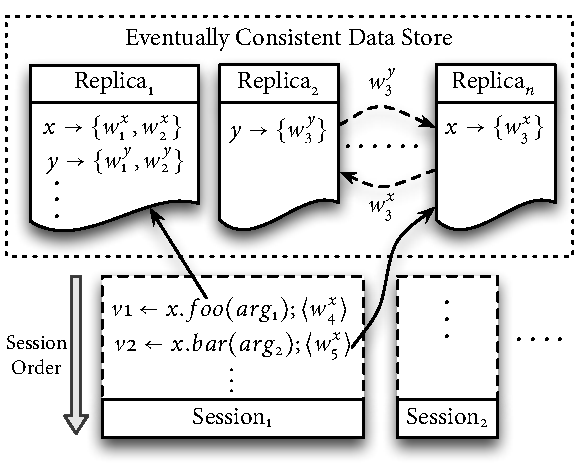
\includegraphics[width=0.65\columnwidth]{Figures/SystemModel}
\caption{\quelea system model.}
\label{fig:sysmod}
\end{figure}

Figure~\ref{fig:sysmod} provides a schematic diagram of our system model. The
distributed store is composed of a collection of \emph{replicas}, each of which
stores a set of \emph{objects} ($x,y,\ldots$). We assume that every object is
replicated at every replica in the store. The state of an object at any replica
is the set of all updates (\emph{effects}) performed on the object. For
example, the state of $x$ at replica 1 is the set composed of effects $w^x_1$
and $w^x_2$.

Each object is associated with a set of \emph{operations}. The clients interact
with the store by invoking operations on objects. The sequence of operations
invoked by a particular client on the store is called a \emph{session}. The
data store is typically accessed by a large number of clients (and hence
sessions) concurrently. Importantly, the clients are oblivious to which replica
an operation is applied to; the data store may choose to route the operation to
any replica in order to minimize latency, balance load, etc. For example, the
operations \emph{foo} and \emph{bar} invoked by the same session on the same
object, might end up being applied to different replicas because replica 1 (to
which \emph{foo} was applied) might be unreachable when the client invokes
\emph{bar}.

When \emph{foo} is invoked on a object $x$ with arguments \emph{arg}$_1$ at
replica 1, it simply \emph{reduces} over the current set of effects at that
replica on that object ($w^x_1$ and $w^x_2$), produces a result $v1$ that is
sent back to the client, and emits a \emph{single} new effect $w^x_4$ that is
appended to the state of $x$ at replica 1. Thus, every operation is evaluated
over a \emph{snapshot} of the state of the object on which it is invoked. In
this case, the effects $w^x_1$ and $w^x_2$ are \emph{visible} to $w^x_4$,
written logically as $\vis{w^x_1}{w^x_4} \wedge \vis{w^x_2}{w^x_4}$, where
$\visZ$ is the visibility relation between effects. Visibility is an
irreflexive and asymmetric relation, and only relates effects produced by
operations on the same object. Executing a read-only operation is similar
except that no new effects are produced.

The effect added to a particular replica is asynchronously sent to other
replicas, and eventually merged into all other replicas. Two effects $w^x_4$
and $w^x_5$ that arise from the same session are said to be in \emph{session
order} (written logically as $\so{w^x_4}{w^x_5}$). Session order is an
irreflexive, transitive relation. The effects $w^x_4$ and $w^x_5$ arising from
operations applied to the same object $x$ are said to be under the \emph{same
object} relation, written $\sameobj{w^x_4}{w^x_5}$. Finally, we can associate
every effect with the operation that generated the effect with the help of a
relation $\operZ$. In the current example, $\oper{w^x_4}{foo}$ and
$\oper{w^x_5}{bar}$ hold. For simplicity, we assume all operation names across
all object types are distinct.

This model admits all the inconsistencies associated with eventual consistency.
The goal of this work is to identify the precise consistency level for each
operation such that application-level constraints are not violated. In the next
section, we will concretely describe the challenges associated with
constructing a consistent bank account on top of an eventually consistent data
store. Subsequently, we will illustrate how our contract and specification
language, armed with the primitive relations $\visZ$, $\soZ$, $\sameobjZ$ and
$\operZ$, mitigates these challenges.

\section{Motivation}
\label{q_sec:motivation}

Consider how we might implement a highly available bank account on top of an
eventually consistent data store, with the \emph{integrity} constraint that the
balance must be non-negative. We begin by implementing a bank account
replicated data type (RDT) in \quelea, and then describe the mechanisms to
obtain the desired correctness guarantees.

\subsection{RDT specification}

A key novelty in \quelea is that it allows the addition of new RDTs to the
store, which obviates the need for coercing the application logic to utilize
the store provided data types. In addition, \quelea treats the convergence
semantics of the data type separately from its consistency properties. This
separation of concerns permits \emph{operational} reasoning for conflict
resolution, and \emph{declarative} reasoning for consistency. The combination
of these techniques enhances the programmability of the store.

Let us assume that the bank account object provides three operations:
\cf{deposit}, \cf{withdraw} and \cf{getBalance}, with the assumption that the
withdraw fails if the account has insufficient balance. Every operation in
\quelea is of the following type, written in Haskell syntax:

\begin{codehaskell}
type Operation = [e] -> a -> (r, Maybe e)
\end{codehaskell}

\noindent It takes a list of effects (the \emph{context} for the operation),
and an input argument, and returns a result along with an optional effect
(read-only operations return \cf{Nothing}). The new effect (if emitted) is
added to the state of the object at the current replica, and asynchronously
sent to other replicas. The implementation of the bank account operations in
\quelea is given in Figure~\ref{fig:ex}:

\begin{figure}
\begin{codehaskell}
data Acc = Deposit Int | Withdraw Int | GetBalance

getBalance :: [Acc] -> () -> (Int, Maybe Acc)
getBalance ctxt _ =
  let res = sum [x | Deposit x <- ctxt]
						- sum [x | Withdraw x <- ctxt]
	in (res, Nothing)

deposit :: [Acc] -> Int -> ((), Maybe Acc)
deposit _ amt = (amt, Just dollar Deposit amt)

withdraw :: [Acc] -> Int -> (Bool, Maybe Acc)
withdraw ctxt v =
	if sel1 dollar getBalance ctxt () >= v
  then (True, Just dollar Withdraw v)
	else (False, Nothing)
\end{codehaskell}
\caption{Definition of a bank account expressed in Quelea.}
\label{fig:ex}
\end{figure}

The datatype \cf{Acc} represents the effect type for the bank account. The
context of the operations is a snapshot of the state of the object at some
replica. In this sense, every operation on the RDT is atomic, and thus
permitting sequential reasoning for implementing eventually consistent data
types. We have implemented a large corpus of RDTs for realistic benchmarks
including shopping carts, auction and micro-blogging sites in few tens of lines
of code.

\subsection{Anomalies under Eventual Consistency}

Our goal is to choose the correct consistency level for each of the bank
account operations such that (1) the balance remains non-negative and (2) the
\cf{getBalance} operation never incorrectly returns a negative balance. Let us
first consider the anomalies that could arise under eventual consistency.

\begin{figure}
\centering
\subfigure[Unsafe withdraw]{\label{fig:unsafeWithdrawAnomaly}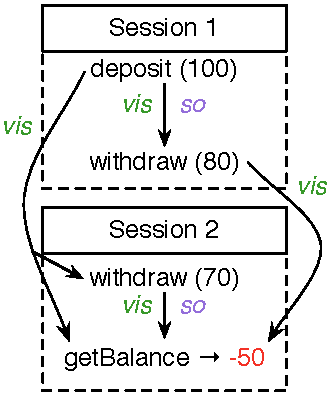
\includegraphics[width=0.34\columnwidth]{Figures/Motivation4}}
\hfill
\subfigure[Negative balance]{\label{fig:negativeBalanceAnomaly}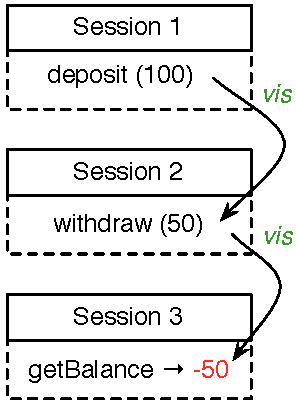
\includegraphics[width=0.31\columnwidth]{Figures/Motivation2}}
\hfill
\subfigure[Missing update]{\label{fig:missingUpdateAnomaly}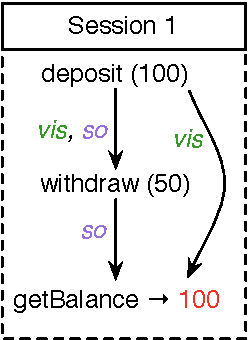
\includegraphics[width=0.26\columnwidth]{Figures/Motivation1}}
\caption{Anomalies possible under eventual consistency for the get balance operation.}
\label{fig:ba_anomalies}
\end{figure}

Consider the execution shown in Figure~\ref{fig:unsafeWithdrawAnomaly}. Assume
that all operations in the figure are on the same bank account object with the
initial balance being zero. Session 1 performs a \cf{deposit} of 100, followed
by a \cf{withdraw} of 80 in the same session. The \cf{withdraw} operation
witnesses the deposit and succeeds\footnote{Although visibility and session
order relations relate effects, we have abused the notation in these examples
to relate operations, with the idea that the relations relate the effect
emitted by those operations}. Subsequently, session 2 perform a \cf{withdraw}
operation, but importantly, due to eventual consistency, only witnesses the
\cf{deposit} from session 1, but not the subsequent withdraw. Hence, this
\cf{withdraw} also \emph{incorrectly} succeeds, violating the integrity
constraint. A subsequent \cf{getBalance} operation, that happens to witness all
the previous operations, would report a negative balance.

It is easy to see that preventing concurrent \cf{withdraw} operations
eliminates this anamoly. This can be done by insisting that \cf{withdraw} be
executed as a strongly consistent operation. Despite this strengthening,
\cf{getBalance} operation may incorrectly report a negative balance to the end
user. Consider the execution shown in fig.~\ref{fig:negativeBalanceAnomaly},
which consists of three concurrent sessions performing a \cf{deposit}, a
\cf{withdraw}, and a \cf{getBalance} operation, respectively, on the same bank
account object. As the \cf{vis} edge indicates, operation \cf{withdraw(50)} in
session 2, witnesses the effects of \cf{deposit(100)} from session 1, concludes
that there is sufficient balance, and completes successfully. However, the
\cf{getBalance} operation may only witness this successful withdraw, but not
the causally preceding \cf{dopsit}, and reports the balance of negative 50 to
the user.

Under eventual consistency, the users may also be exposed to other forms of
inconsistencies. Figure~\ref{fig:missingUpdateAnomaly} shows an execution where
the \cf{getBalance} operation in a session does not witness the effects of an
earlier \cf{withdraw} operation performed in the same session, possibly because
it was served by a replica that has not yet merged the \cf{withdraw} effect.
This anomaly leads the user to incorrectly conclude that the \cf{withdraw}
operation failed to go through.

Although it is easy to understand the reasons behind the occurrence of the
aforementioned anomalies, finding the appropriate fixes is not readily
apparent. Making \cf{getBalance} a strongly consistent operation is definitely
sufficient to avert anomalies, but is it really necessary? Given the cost of
enforcing strong consistency~\cite{DynamoDB,Terry2013}, it is preferable to avoid
it unless there are no viable alternatives. Exploring the space of these
alternatives requires understanding the subtle differences in semantics of
various kinds of weak consistency alternatives.

\subsection{Contracts}

\quelea helps facilitate the mapping of operations to appropriate consistency
levels by letting the programmer declare application-level consistency
constraints as \emph{contracts}
(Figure~\ref{fig:contract-lang}\footnote{\quelea exposes the contract
construction language as a Haskell library}) that axiomatically specify the set
of allowed executions involving this operation. In the case of the bank
account, any execution that does not exhibit the anomalies described in the
previous section is a \emph{well-formed} execution on the bank account object.
By specifying the set of legal executions for each data type in terms of a
trace of operation invocations on that type, \quelea\ ensures that all
executions over that type are well-formed.

In our running example, it is clear that in order to preserve the integrity
constraint, the \cf{withdraw} operation must be strongly consistent.  That is,
given two \cf{withdraw} operations $a$ and $b$, either $a$ is visible to $b$ or
vice versa. We express this application-level consistency requirement as a
contract ($\cv_w$) over \cf{withdraw}:
\begin{mathpar}
\begin{array}{l}
\forall (a : \rcf{withdraw}).~\sameobj{a}{\cureff} \Rightarrow a = \cureff \vee \vis{a}{\cureff} \vee \vis{\cureff}{a}
\end{array}
\end{mathpar}

\noindent Here, $\cureff$ stands for the effect emitted by the \cf{withdraw} operation.
The syntax $a:\rcf{withdraw}$ states that $a$ is an effect  emitted
by a \cf{withdraw} operation i.e., $\oper{a}{\rcf{withdraw}}$ holds.  The
contract specifies that if the current operation emits an effect $\cureff$,
then for any operation $a$ which was emitted by a \cf{withdraw} operation, it
is the case that $a = \cureff$ or $a$ is visible to $\cureff$, or vice versa.
Any execution on a bank account object that preserves the above contract for a
\cf{withdraw} operation is said to be derived from a correct implementation of
\cf{withdraw}.

\noindent For \cf{getBalance}, we construct the following contract ($\cv_{gb}$):
\begin{mathpar}
\begin{array}{l}
\forall (a:\rcf{deposit}), (b:\rcf{withdraw}), (c: \rcf{deposit} \vee \rcf{withdraw}). \\
\qquad \vis{a}{b} \wedge \vis{b}{\cureff} \Rightarrow \vis{a}{\cureff} \\
\qquad \wedge~ (\soZ \cap \sameobjZ) (c,\cureff) \Rightarrow \vis{c}{\cureff}
\end{array}
\end{mathpar}

\noindent The expression $c:\rcf{deposit} \vee \rcf{withdraw}$ states that $c$
is an effect that was emitted either by a \cf{deposit} or a \cf{withdraw}
operation. If a \cf{withdraw} $b$ is visible to \cf{getBalance} $\cureff$, then
all \cf{deposit} operations $a$ visible to $b$ should also be visible to
$\cureff$. This prevents negative balance anomalies. Our contract language
provides operators to compose relations. The syntax $(R_1 \cap R_2)(a,b)$ is
equivalent to $R_1(a,b) \wedge R_2(a,b)$. The last line of the above contract
says that if a \cf{deposit} or a \cf{withdraw} operation precedes a
\cf{getBalance} operation in session order, and is applied on the same object
as the \cf{getBalance} operation, then it must be the case that the
\cf{getBalance} operation witnesses the effects of the preceding operations.

Finally, since there are no restrictions on when or how a \cf{deposit}
operation can execute, its contract is simply $\small \true$.

\subsection{From Contracts to Implementation}

Notice that the contracts for \cf{withdraw} and \cf{getBalance} only express
application-level consistency requirements, and make no reference to the
semantics of the underlying store. To write contracts, a programmer only needs
to reason about the semantics of the application under the \quelea system model.
The mapping of application-level consistency requirements to appropriate
store-level guarantees is done automatically behind-the-scene. How might one go
about ensuring that an execution adheres to a contract? The challenge is that a
contract provides a declarative (axiomatic) specification of an execution,
while what is required is an operational procedure for \emph{enforcing} its
implicit constraints.

One strategy would be to execute operations speculatively.  Here, operations
are tentatively applied as they are received from the client or other replicas.
We can maintain a runtime manifestation of executions, and check
well-formedness conditions at runtime, rolling back executions if they are
ill-formed. However, the overhead of state maintenance and the complexity of
user-defined contracts is likely to make this technique infeasible in practice.

We devise a static approach instead. Contracts are analyzed with the help of a
theorem prover, and statically mapped to a particular store-level consistency
property that the prover guarantees preserves contract semantics. We call this
procedure \emph{contract classification}. Given the variety and complexity of
store level consistency properties, the idea is that the system implementor
parameterizes the classification procedure by describing the store semantics in
the \emph{same} contract language as the one used to express the contract on
the operations. In the next section, we describe the contract language in
detail and describe the classification procedure for a particular store
semantics.

\section{Contract Language}
\label{q_sec:lang}

\begin{figure}[t]
\begin{mathpar}
\begin{array}{rclcl}
\multicolumn{5}{l}{
  {x,y,z} \in \mathtt{EffVar} \qquad
  {\cureff} \in \mathtt{CurEff} \qquad
  {\sf Op} \in \mathtt{OperName}
}\\
\cv 		& \in & \mathtt{Contract} 	& \coloneqq & \forall (x : \tau).\cv
        \ALT \pi \\
\tau		& \in	& \mathtt{EffType}	& \coloneqq &  {\sf Op}
        \ALT \tau \vee \tau \\
\pi			&	\in & \mathtt{Prop} & \coloneqq & \true \ALT R(x,y)
        \ALT \pi \vee \pi \\
			  & 		&	 &  \ALT & \pi \wedge \pi \ALT \pi \Rightarrow \pi \\
R				& \in & \mathtt{Relation}	& \coloneqq & \visZ \ALT \soZ
        \ALT \sameobjZ \ALT R^+ \\
				&			&	 &  \ALT & R \cup R \ALT R \cap R \\
\end{array}
\end{mathpar}
\caption{Contract language.}
\label{fig:contract-lang}
\end{figure}

\subsection{Syntax}

The syntax of our core contract language is shown in Figure
~\ref{fig:contract-lang}. The language is based on first-order logic (FOL), and
admits prenex universal quantification over typed effect variables. We use a
special effect variable ($\cureff$) to denote the effect of \emph{current
operation} - the operation for which a contract is being written. The type of
an effect is simply the name of the operation (eg: \cf{withdraw}) that induced
the effect. We admit disjuntion in types to let an effect variable range over
multiple operation names. The contract $\small \forall (a : \tau_1 \vee
\tau_2).~\psi$ is just syntactic sugar for $\small \forall a. (\oper{a}{\tau_1}
\vee \oper{a}{\tau_2}) \Rightarrow \psi$.

Quantifier-free propositions in our contract language are conjunctions,
disjunctions and implications of predicates expressing relations between pairs
of effect variables. The syntactic class of relations is seeded with primitive
$\visZ$, $\soZ$, and $\sameobjZ$ relations, and also admits derived relations
that are expressible as union, intersection, or transitive closure. Strictly
speaking, $R^{+}$ is not the transitive closure of $R$, as transitive closure
is not expressible in FOL.  Instead, $R^{+}$ in our language denotes \emph{a}
superset of transitive closure of $R$. Formally, $R^{+}$ is any relation $R'$
such that forall $x$, $y$, and $z$, a) $R(x,y) \Rightarrow R'(x,y)$, and b)
$R'(x,y) \conj R'(y,z) \Rightarrow R'(x,z)$ of primitive relations.  Commonly
used derived relations are:

\begin{itemize}

\item Same object session order: $\sooZ = \soZ ~\cap~ \sameobjZ$.

\item Happens-before order: $\hbZ = (\soZ ~\cup~ \visZ)^+$.

\item Same object happens-before order: $\hboZ = (\sooZ ~\cup~ \visZ)^+$.

\end{itemize}

\subsection{Semantics}

\begin{figure}[t]
\begin{mathpar}
\begin{array}{lclcl}
\multicolumn{5}{l}{
  {\eff} \in \mathtt{Effect} \qquad
  {\cv} \in \mathtt{Contract} \qquad
  \set{\eff} \in \mathtt{Effect\; Set}
}\\
\EffSoup & \in & \mathtt{EffSoup}	  & \coloneqq & \set{\eff} \\
\visZ, \soZ, \sameobjZ &	\in & \mathtt{Relations} & \coloneqq & \EffSoup \times \EffSoup \\
%\sameobjZ		&     &  & \\
{\E} 		& \in & \mathtt{ExecState}  & \coloneqq & \Exec \\
\end{array}
\end{mathpar}

\caption{Axiomatic execution.}
\label{sem:ax_ex}
\end{figure}

\quelea contracts are constraints over axiomatic definitions of program
executions. Figure~\ref{sem:ax_ex} summarizes artifacts relevant to define
an axiomatic execution. We formalize an axiomatic execution as a tuple $\Exec$,
where $\EffSoup$, called the \emph{effect soup}, is the set of all effects
generated during the program execution, and $\visZ,\soZ,\sameobjZ \subseteq
\EffSoup \times \EffSoup$ are \emph{visibility}, \emph{session order}, and
\emph{same object} relations, respectively, witnessed over generated effects at
run-time.

Note that the axiomatic definition of an execution ($\E$) provides
interpretations for primitive relations (eg: $\visZ$) that occur free in
contract formulas, and also fixes the domain of quantification to set of all
effects ($\EffSoup$) observed during the program execution. As such, $\E$ is a
potential model for any first-order formula ($\cv$) expressible in our contract
language. If $\E$ is indeed a valid model for $\cv$ (expressed using the
model-theoretic consequence relation as $\E \models \cv$), we say that the
execution $\E$ satisfied the contract $\cv$:

\begin{definition}
An axiomatic execution $\E$ is said to satisfy a contract $\cv$ if and only if
$\E \models \cv$.
\end{definition}

\subsection{Capturing Store Semantics}
\label{q_sec:store_sem}

An important aspect of our contract language is its ability to capture
store-level consistency guarantees, along with application-level consistency
requirements. Similar to~\cite{Burckhardt2014}, we can rigorously define a wide
variety of store semantics including those that combine any subset of session
and causality guarantees, and multiple consistency levels.  However, for our
purposes, we identify three particular consistency levels -- eventual, causal,
and strong, commonly offered by many distributed stores with tunable
consistency, with increasing overhead in terms of latency and availability.

\begin{itemize}
\setlength{\itemsep}{2pt}

\item \textbf{Eventually consistency}: Eventually consistent operations can
	be satisfied as long as the client can reach at least one replica. In the
	bank account example, \cf{deposit} is an eventually consistent operation.
	While eventually consistent data stores typically offer \emph{basic} eventual
	consistency with all possible anomalies, we assume that our store provides
	stronger semantics that remain highly-available~\cite{BailisHAT,COPS}; the
	store always exposes a \emph{causal cut} of the updates. This semantics can
	be formally captured in terms of the following contract definition:
  \begin{mathpar}
  \ecc = \forall a,b. ~\hbo{a}{b} \wedge \vis{b}{\cureff} \Rightarrow \vis{a}{\cureff}
  \end{mathpar}

\item \textbf{Causal consistency}: Causally consistent operations are required
	to see a causally consistent snapshot of the object state, including the
	actions performed on the same session.  The latter requirement implies that
	if two operations $o_1$ and $o_2$ from the same session are applied to two
	different replicas $r_1$ and $r_2$, the second operation cannot be discharged
	until the effect of $o_1$ is included in $r_2$. The \cf{getBalance} operation
	requires causal consistency, as it requires the operations from the same
	session to be visible, which cannot be guaranteed under eventual consistency.
	The corresponding store semantics is captured by the contract $\ccc$ defined
	below:
  \begin{mathpar}
  \ccc = \forall a.~\hbo{a}{\cureff} \Rightarrow \vis{a}{\cureff}
  \end{mathpar}

\item \textbf{Strong Consistency}: Strongly consistent operations may block
  indefinitely under network partitions. An example is the total-order
  contract on \cf{withdraw} operation. The corresponding store semantics is
	captured by the $\scc$ contract definition:
  \begin{mathpar}
  \scc = \forall a.~\sameobj{a}{\cureff} \Rightarrow \vis{a}{\cureff} ~\vee~ \vis{\cureff}{a} ~\vee~ a = \cureff
  \end{mathpar}

\end{itemize}

\newcommand{\DDe}[1]{#1}
\begin{figure}[t]
\begin{mathpar}
\begin{array}{c}
\RuleTwo
{\DDe{\cv} \le \DDe{\scc}}
{{\sf WellFormed}(\cv)}  \qquad

\RuleTwo
{\DDe{\cv} \le \DDe{\ecc}}
{{\sf EventuallyConsistent}(\cv)} \\ \\

\RuleTwo
{\DDe{\cv} \not\le \DDe{\ecc}
\quad \DDe{\cv} \le \DDe{\ccc}}
{{\sf CausallyConsistent}(\cv)} \qquad

\RuleTwo
{\DDe{\cv} \not\le \DDe{\ccc}
\quad \DDe{\cv} \le \DDe{\scc}}
{{\sf StronglyConsistent}(\cv)}

\end{array}
\end{mathpar}
\caption{Contract classification.}
\label{sem:classify}
\end{figure}

\subsection{Contract Comparison and Classification}

Our goal is to map application-level consistency constraints on operations to
appropriate store-level consistency guarantees capable of satisfying these
constraints.  The ability to express both these kinds of constraints as
contracts in our contract language lets us compare and determine if contract
($\cv_{op}$) of an operation ($\mathit{op}$) is weak enough to be satisfied
under a store consistency level identified by the contract $\cv_{st}$. Towards
this end, we define a binary \emph{weaker than} relation for our contract
language as following:

\begin{definition}
A contract $\cv_{op}$ is said to be weaker than $\cv_{st}$ (written $\cv_{op}
\le \cv_{st}$ ) if and only if $\Delta \vdash \cv_{st} \Rightarrow \cv_{op}$.
\end{definition}

The $\Delta$ referred in the above defintion is a conjunction of assumptions
about the nature of primitive relations. A \emph{well-formed} axiomatic
execution ($\E$) is expected to satisfy these assumptions (i.e., $\E \models
\Delta$).

\begin{definition}
An axiomatic executions $\E = \Exec$ is said to be well-formed if the following
axioms ($\Delta$) hold:

\begin{itemize}
\item The happens-before relation is acyclic: $\forall a.~\neg\hb{a}{a}$.
\item Visibility only relates actions on the same object: $\forall a,b.~\vis{a}{b} \Rightarrow \sameobj{a}{b}$.
\item Session order is a transitive relation: $\forall a,b,c.~\so{a}{b} ~\wedge~ \so{b}{c} \Rightarrow \so{a}{c}$.
\item Same object is an equivalence relation:
	\begin{itemize}
	\item $\forall a.~\sameobj{a}{a}$.
	\item $\forall a,b.~\sameobj{a}{b} \Rightarrow \sameobj{b}{a}$.
	\item $\forall a,b,c.~\sameobj{a}{b} ~\wedge~ \sameobj{b}{c} \Rightarrow \sameobj{a}{c}$.
	\end{itemize}
\end{itemize}
\end{definition}

If the contract ($\cv_{op}$) of an operation ($\mathit{op}$) is \emph{weaker
than} a store contract ($\cv_{st}$), then constraints expressed by the former
are implied by guarantees provided by the latter. The completeness of
first-order logic allows us to assert that any well-formed execution ($\E$)
that satisfies $\cv_{st}$ (i.e., $\E\models \cv_{st}$) also satisfies
$\cv_{op}$ (i.e., $\E \models \cv_{op}$). Consequently, it is safe to execute
operation $\mathit{op}$ under a store consistency level captured by $\cv_{st}$.

Observe that the contracts $\scc$, $\ccc$ and $\ecc$ are themselves totally
ordered with respect to the $\le$ relation: $\ecc \le \ccc \le \scc$.  This
concurs with the intuition that any contract satisfiable under $\ecc$ or $\ccc$
is satisfiable under $\scc$, and any contract that is satisfiable under $\ecc$
is satisfiable under $\ccc$. We are interested in the \emph{weakest} guarantee
(among $\ecc$, $\ccc$, and $\scc$) required to satisfy the contract. We define
the corresponding consistency level as the \emph{consistency class} of the
contract.

The classification scheme, presented formally in Figure~\ref{sem:classify},
defines rules to judge the consistency class of a contact. For example, the
scheme classifies the \cf{getBalance} contract ($\cv_{gb}$) from
Section~\ref{q_sec:motivation} as a {\sf\small CausallyConsistent} contract, because
the sequent $\Delta \vdash \ccc \Rightarrow \cv_{gb}$ is valid in first-order
logic (therefore, $\cv_{gb} \le \ccc$), whereas the sequent $\Delta \vdash \ecc
\Rightarrow \cv_{gb}$ is invalid (therefore, $\cv_{gb} \not\le \ecc$). Since we
confine of our contract language to a decidable subset of the logic, validity
of such sequents can be decided mechanically allowing us to automate the
classification scheme in \quelea.

Along with three straightforward rules that classify contracts into consistency
classes, the classification scheme also presents a rule that judges
well-formedness of a contract. A contract is well-formed if and only if it is
satisfiable under $\scc$ - the strongest possible consistency guarantee that
the store can provide. Otherwise, it is considered ill-formed, and rejected
statically.

\subsection{Soundness of Contract Classification}

We now present a meta-theoretic result that certifies the soundness of
classification-based contract enforcement. To help us state the result, we
define an operational semantics of the our system described informally in
Section~\ref{q_sec:sysmod}:
\begin{mathpar}
\begin{array}{lclcl}
{\it op} 	& \in & \mathtt{Operation} \\
{\tau}		& \in & \mathtt{Consistency Class} 	& \coloneqq & {\sf ec},{\sf cc},{\sf sc} \\
{\sigma} 	& \in & \mathtt{Session} 					 	& \coloneqq & \cdot \ALT \langle op,\tau \rangle; \sigma \\
\Sigma 		& \in & \mathtt{Session\;Soup}   	 	& \coloneqq & \sigma \pll \Sigma \ALT \emptyset \\
					&			&	\mathtt{Config}		  			 	& \coloneqq & \E,\Sigma \\
\end{array}
\end{mathpar}

We model the system as a tuple $\E,\Sigma$, where the axiomatic execution $\E$
captures the data store's current state, and session soup $\Sigma$ is the set
of concurrent client sessions interacting with the store. A session $\sigma$ is
a sequence of pairs composed of replicated data type operations $\mathit{op}$,
tagged with the consistency class $\tau$ of their contracts (as determined by
the contract classification scheme). We assume a reduction relation of form:
\begin{mathpar}
  \auxred{} {\E,\langle op,\tau \rangle;\sigma \pll \Sigma} {\eff}
    {\E',\sigma \pll \Sigma}
\end{mathpar}

\noindent on the system state. The relation captures the progress of the
execution (from $\E$ to $\E'$)  due to the successful completion of a client
operation $\mathit{op}$ from one of the sessions in $\Sigma$, generating a new
effect $\eff$. If the resultant execution $\E'$ satisfies the store contract
$\cv_\tau$ (i.e., $\E \models \cv_\tau$), then we say that the store has
\emph{enforced} the contract $\cv_\tau$ in the execution $\E'$. With help of
the operational semantics, we now state the soundness of contract enforcement
as follows:

\begin{theorem}[Soundness of Contract Enforcement]
\label{thm:classification-sound}
Let $\cv$ be a well-formed contract of a replicated data type operation
$\mathit{op}$, and let $\tau$ denote the consistency class of $\cv$ as
determined by the contract classification scheme. For all well-formed execution
states $\E$, $\E'$ such that
$\auxred{} {\E,\langle op,\tau \rangle;\sigma \pll \Sigma} {\eff} {\E', \sigma
\pll \Sigma}$, if $\E' \models \cv_\tau[\eff/\cureff]$, then $\E' \models
\cv[\eff/\cureff]$
\end{theorem}

\noindent The theorem states that if a data store correctly enforces $\scc$,
$\ccc$, and $\ecc$ contracts in all well-formed executions, then the same
store, extended with the classification scheme shown in
Figure~\ref{sem:classify}, can enforce all well-formed \quelea contracts. The
proof of the theorem along with the operational semantics for store that
provides multiple consistency levels is presented in the next section.

\section{Operational Semantics}
\label{q_sec:meta-theory}

\section{Transaction Contracts}
\label{q_sec:txns}

While contracts on individual operations offer the programmer object-level
declarative reasoning, real-world scenarios often involve operations that span
multiple objects. In order to address this problem, several recent
systems~\cite{Walter,Burckhardt2012,BailisHAT} have proposed eventually
consistent transactions in order to compose operations on multiple objects.
However, given that classical transaction models such as serializability and
snapshot isolation require inter-replica coordination, these systems espouse
\emph{coordination-free transactions} that remain available under network
partitions, but only provide weaker isolation guarantees. Coordination-free
transactions have intricate consistency semantics and widely varying runtime
overheads. As with operation-level consistency, the onus is on the programmer
to pick the correct transaction kind. This choice is further is complicated by
consistency semantics of individual operations.

\subsection{Syntax and Semantics Extension}
\label{q_sec:syn_sem_ext}

\quelea automates the choice of assigning the correct and most efficient
transaction isolation level. Similar to contracts on individual operations, the
programmer associates contracts with transactions, declaratively expressing its
consistency specification. We extend the contract language with a new term
under quantifier-free propositions - ${\small \txnZ}~S_1~S_2$, where $S_1$ and
$S_2$ are sets of effects, and introduce a new primitive equivalence relation
$\small \sametxnZ$ that holds for effects from the same transaction. $\small
\txn{a,b}{c,d}$ is just syntactic sugar for $\small \sametxn{a}{b} ~\wedge~
\sametxn{c}{d} ~\wedge~ \neg\sametxn{a}{c}$, where $a$ and $b$ considered to
belong to the \emph{current} transaction.

We assume that operations not part of any transaction belong to their own
unique transaction. While transactions may have varying isolation guarantees,
we make the standard assumption that all transactions provide atomicity. Hence,
we include the following axioms in $\Delta$:

\begin{itemize}
\item Same transactions is an equivalence relation:
	\begin{itemize}
	\item $\forall a.~\sametxn{a}{a}$.
	\item $\forall a,b.~\sametxn{a}{b} \Rightarrow \sametxn{b}{a}$.
	\item $\forall a,b,c.~\sametxn{a}{b} ~\wedge~ \sametxn{b}{c} \Rightarrow \sametxn{a}{c}$.
	\end{itemize}
\item Atomicity of transaction:
	\begin{itemize}
	\item $\forall a,b,c.~\txn{a}{b,c} ~\wedge~ \sameobj{b}{c} ~\wedge~ \vis{b}{a} \Rightarrow \vis{c}{a}$.
	\end{itemize}
\item Transaction does not span across sessions:
	\begin{itemize}
	\item $\forall a,b.~\sametxn{a}{b} \Rightarrow \so{a}{b} ~\vee~ \so{b}{a} ~\vee~ a = b$.
	\end{itemize}
\item Transactions are contiguous:
	\begin{itemize}
	\item $\forall a,b,c~\sametxn{a}{c} ~\wedge~ \so{a}{b} ~\wedge~ \so{b}{c} \Rightarrow \sametxn{a}{b}$.
	\end{itemize}
\end{itemize}

\noindent The semantics of the atomicity axiom is illustrated in
Figure~\ref{fig:txn_atomicity}.

\subsection{Transactional Bank Account}

In order to illustrate the utility of declarative reasoning for transactions,
consider an extension of our running example to use two accounts (objects) --
current ($c$) and savings ($s$). Each account provides operations
\cf{withdraw}, \cf{deposit} and \cf{getBalance}, with the same contracts as
defined previously. We consider two transactions -- \cf{save(amt)}, which
transfers \cf{amt} from current to savings, and \cf{totalBalance}, which
returns the sum of the balances of individual accounts. The \quelea code for the
transactions is given below:

\hspace{1em}
\begin{minipage}[t]{0.4\columnwidth}
\begin{codehaskell}
save amt =
  x <- dollar(classify $\cv_{sv}$)
  atomically x dollar do
    b <- withdraw c amt
    when b dollar deposit s amt
\end{codehaskell}
\end{minipage}
\hfill
\begin{minipage}[t]{0.4\columnwidth}
\begin{codehaskell}
totalBalance =
  x <- dollar(classify $\cv_{tb}$)
  atomically x dollar do
    b1 <- getBalance s
    b2 <- getBalance s
    return b1 + b2
\end{codehaskell}
\end{minipage}
\hspace{1em}

$\cv_{sv}$ and $\cv_{tb}$ are the contracts on the corresponding
transactions. The function \cf{classify} assigns the contracts
\emph{statically} to one of the transaction isolation levels offered by the
store; \cf{\$()} is meta-programming syntax for splicing the result into the
program. The \cf{atomically} construct invokes the enclosing operations at the
given isolation level $x$, ensuring that the effects of the operations are made
visible atomically. Our goal is to ensure that \cf{totalBalance} returns the
result obtained from a consistent snapshot of the object states.

While making both transactions serializable would ensure correctness,
distributed stores rarely offer serializable transactions since it is
unavailable and hinders scalability~\cite{BailisHAT}. As we will see, these
transactions can be satisfied with much weaker isolation guarantees. Despite
the atomicity offered by the transaction, anomalies are still possible. For
example, the two \cf{getBalance} operations in \cf{totalBalance} transactions
might be served by different replicas with distinct set of committed \cf{save}
transactions. If the first(second) \cf{getBalance} operation witness a
\cf{save} transaction that is not witnessed by the second(first)
\cf{getBalance} operation, then the balance returned will be less(greater) than
the actual balance. It is not immediately apparent which weakest isolation
guarantee will be sufficient to prevent the anomaly.

Instead, \quelea requires the programmer to simply state the consistency
requirement as a contract. Since we would like both the \cf{getBalance}
operations to witness the same set of \cf{save} transactions, we define the
constraint on \cf{totalBalance} transaction $\psi_{tb}$ as:
\begin{mathpar}
\begin{array}{l}
\cv_{tb} = \forall a:\rcf{getBalance}, b:\rcf{getBalance}, \\
\quad \qquad (c:\rcf{withdraw} \vee \rcf{deposit}), (d:\rcf{withdraw} \vee \rcf{deposit}). \\
\quad \qquad \txn{a,b}{c,d} ~\wedge~ \vis{c}{a} ~\wedge~ \sameobj{d}{b} \Rightarrow \vis{d}{b}
\end{array}
\end{mathpar}

\noindent The key idea in the above definition is that the $\txnZ$ primitive
allows us to relate operations on different objects. The \cf{save} transaction
only needs to ensure that the two writes it performs are made visible
atomically. Since this is ensured by combining them in a transaction, \cf{save}
does not require any additional constraints, and $\psi_1$ is simply $\small
\true$.

\subsection{Coordination-free Transactions}

\begin{figure}[t]
\centering
\subfigure[Atomicity]{\label{fig:txn_atomicity}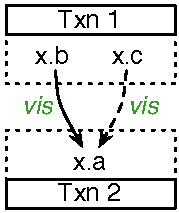
\includegraphics[width=0.3\columnwidth]{Figures/TxnAtomic}}
\hfill
\subfigure[Monotonic Atomic View]{\label{fig:txn_mav}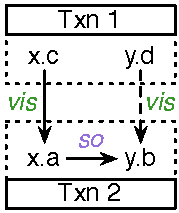
\includegraphics[width=0.3\columnwidth]{Figures/TxnMAV}}
\hfill
\subfigure[Repeatable Read]{\label{fig:txn_rr}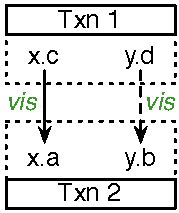
\includegraphics[width=0.3\columnwidth]{Figures/TxnRR}}
\caption{Semantics of transaction contracts. $x$ and $y$ are distinct objects.
The dotted line represents the visibility requested by the contracts.}
\label{fig:transaction}
\end{figure}

In order to illustrate the utility of transaction contract classification, we
identify three well-understood coordination-free transaction semantics -- Read
Committed (RC)~\cite{Berenson95}, Monotonic Atomic View (MAV)~\cite{BailisHAT}
and Repeatable Read (RR)~\cite{Berenson95}, and illustrate the classification
strategy. Our technique can indeed be applied to a different isolation level
lattice.

A transaction with ANSI RC semantics only witnesses committed operations. Let
us assume that the store buffers updates until all the updates from the
transaction are available at a replica. If the transaction commits, the
buffered updates are made visible. Otherwise, the buffered updates are
discarded. RC does not entail any further isolation guarantees. Hence, a store
implementing RC does not require inter-replica coordination. We can express RC
as follows:
\begin{mathpar}
\begin{array}{l}
\rcc = \forall a,b,c.~\txn{a}{b,c} \wedge \sameobj{b}{c} ~\wedge~ \vis{b}{a} \Rightarrow \vis{c}{a}
\end{array}
\end{mathpar}

\noindent Notice that the above definition is the same as the atomicity
guarantee of transaction described in Section~\ref{q_sec:syn_sem_ext}. The
\cf{save} is an example for RC transaction.

MAV semantics ensures that if some operation in a transaction $T_1$ witnesses
the effects of another transaction $T_2$, then subsequent operations in $T_1$
will also witness the effects of $T_2$. MAV semantics is useful for
maintaining the integrity of foreign key constraints, materialized views and
secondary updates. In order to implement MAV, a store only needs to keep track
of the set of transactions $S_t$ witnessed by the running transaction, and
before performing an operation at some replica, ensure that the replica
includes all the transactions in $S_t$. Hence, MAV is coordination-free. MAV
semantics is captured with the following contract:
\begin{mathpar}
\begin{array}{l}
\mavc = \forall a,b,c,d.~\txn{a,b}{c,d} ~\wedge~ \so{a}{b} ~\wedge~ \vis{c}{a} ~\wedge~ \sameobj{d}{b} \Rightarrow \vis{d}{b}
\end{array}
\end{mathpar}

\noindent whose semantics is illustrated in the Figure~\ref{fig:txn_mav}.

ANSI RR semantics requires that the transaction witness a snapshot of the data
store state. Importantly, this snapshot can be obtained from any replica, and
hence RR is coordination-free. An example for such a transaction is the
\cf{totalBalance} transaction. The semantics of RR is captured by the following
contract:
\begin{mathpar}
\begin{array}{l}
\rrc = \forall a,b,c,d.~\txn{a,b}{c,d} ~\wedge~ \vis{c}{a} ~\wedge~ \sameobj{d}{b} \Rightarrow \vis{d}{b}
\end{array}
\end{mathpar}

\noindent whose semantics is illustrated in the Figure~\ref{fig:txn_rr}.

\subsection{Classification}

Similar to operation-level contracts, with respect to $\le$ relation, the
coordination-free transaction semantics described here form a total order:
$\rcc \le \mavc \le \rrc$. The transaction classification is also similar to
the operation-level contract classification presented in
Figure~\ref{sem:classify}; given a contract $\psi$ on a transaction, we start
from the weakest transaction contract $\rcc$, and progressively compare its
strength to the known transaction contracts until we find a isolation level
under which $\psi$ can be safely discharged. Otherwise, we report a type error.

\section{Implementation}
\label{q_sec:impl}

\quelea is implemented as a shallow extension of GHC Haskell and runs on top of
Cassandra, an off-the-shelf eventually consistent distributed data (or backing)
store responsible for all data management issues (i.e., replication, fault
tolerance, availability, and convergence).  Template Haskell is used implement
static contract classification, and proof obligations are discharged with the
help of the Z3~\cite{Z3} SMT solver. Figure~\ref{fig:impl_mod} illustrates the
overall system architecture.

\begin{figure}
\begin{center}
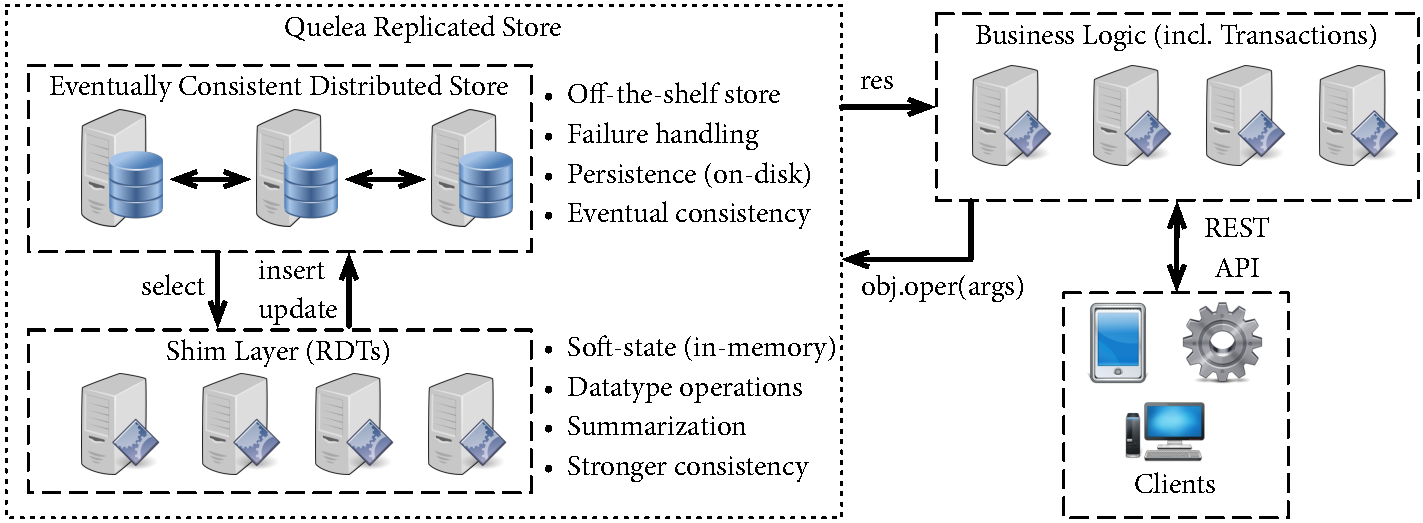
\includegraphics[width=0.7\columnwidth]{Figures/ImplModel}
\end{center}
\caption{Implementation model.}
\label{fig:impl_mod}
\end{figure}

Replicated data types and the stronger consistency semantics are implemented
and enforced in the \emph{shim layer}. Our implementation supports eventual,
causal, and strong consistency for data type operations, and RC, MAV, and RR
semantics for transactions.  This functionality is implemented entirely on top
of the standard interface exposed by Cassandra. From an engineering
perspective, leveraging an off-the-shelf data store enables an implementation
comprising roughly only 2500 lines of Haskell code, which is packaged as a
library.

\subsection{Shim Layer}

The shim layer maintains a causally consistent in-memory snapshot of a subset
of objects in the backing store, by explicitly tracking dependencies introduced
between the effects due to visibility, session and same transaction relations.
The dependence tracking is similar to the techniques presented in~\cite{BoltOn}
and~\cite{Eiger}, with the usual optimizations making use of transitivity
properties for minimizing the number of dependencies. Shim layer performs the
reductions associated with replicated datatype operations corresponding to
client requests. As the backing store provides durability, convergence and
fault tolerance, each shim layer node simply acts as a soft-state cache, and
can safely be terminated at any instant. Similarly, more shim layer nodes can
be spawned on demand.

\subsection{Operation Consistency}

Every effect generated as a result of an effectful operation on an object
inserts a new row $(o,e,vis,txn,val)$ into the backing store, where $o$ and $e$
are object and (unique) effect identifiers, $vis$ is the set of identifiers of
effects visible to this operation, $txn$ is an optional transaction identifier,
and $val$ is the value associated with the effect (eg: \cf{Withdraw 50}). The
shim layer periodically fetches updates from the backing store for those objects
which were accessed since updates were last fetched. Since causally consistent
operations require an up-to-date view of the current session, the shim layer
node synchronously fetches operations if the causally preceding operations in
the current session are not available in the cache.  Strongly consistent
operations are performed after obtaining exclusive leases on objects. The lease
mechanism is implemented with the help of Cassandra's support for conditional
updates and expiring columns.

\subsection{Transactions}

While Cassandra offers all-or-nothing failure semantics for multiple writes
through batching, readers may witness the initial write while the batch is in
progress. \quelea implements atomic visibility by exploiting shim layer causality
guarantee -- an effect is included only if all the effects if depends on are
also included.

\begin{figure}[t]
\begin{center}
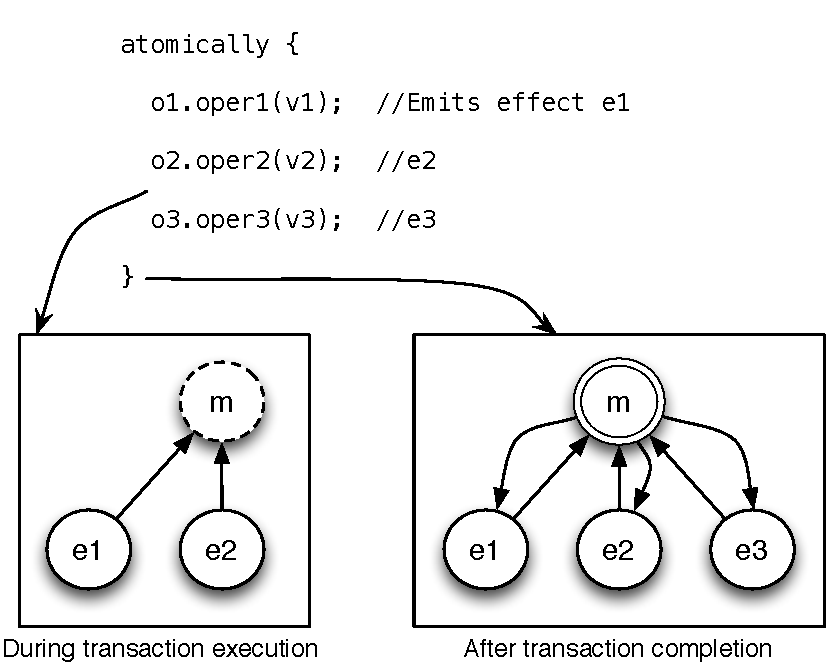
\includegraphics[width=0.7\columnwidth]{Figures/AtomicityImpl}
\end{center}
\caption{Implementing atomicity semantics. Dotted circle represents effects not yet inserted into the backing store.}
\label{fig:atomicity_impl}
\end{figure}

Consider the example given in Figure~\ref{fig:atomicity_impl}. For every
transaction in \quelea, we instantiate a special transaction marker effect $m$.
But importantly, do not insert into the backing store. $m$ is included as a
dependence to every effect generated in the transaction. In the figure, the
graph on the left shows the state of the store in the middle of a transaction.
Each circle represents an effect. The dotted circle indicates that the effect
has been instantiated, but has not yet been inserted into the store. Since the
causally preceding effect $m$ has not yet been written to the store, no
operation will witness $e1$ and $e2$ while the transaction in progress. After
the transaction has finished execution, we insert $m$ into the backing store,
marking all the effects from the transactions as a depedence for $m$. Now any
replica which includes one of the effects from the transaction must include
$m$, and transitively must include every effect from the transaction. This
ensures atomicity and satisfies the RC requirement.

The above scheme prevents a transaction from witnessing its own effects. This
might conflict with the causality requirement on the operations. Hence,
transactions piggy-back the previous effects from the same transaction for each
request. MAV semantics is implemented by keeping track of the set of
transaction markers $M$ witnessed by the transaction, and before performing an
operation at some replica, ensuring that $M$ is a subset of the transaction
markers included at that replica. If not, the missing effects are synchronously
fetched. RR semantics is realized by capturing a optimized snapshot of the
state of some replica; each operation from an RR transaction is applied to this
snapshot state. Any generated effects are added to this snapshot.

\subsection{Summarization}

The main challenge in realizing an efficient implementation of operation-based
replicated data types is that the state of the object i.e., the set of effects
grows with every effectful operation on the object. If left unchecked, the
operations slow down over time, until the shim layer memory or backing store
disk runs out of memory. Luckily, the state of the operation-based replicated
data type can often be summarized to an \emph{observably equivalent} smaller
state. For example,

\begin{itemize}
\setlength{\itemsep}{2pt}
\item A last-writer-wins register with multiple updates where $v$ is the value
of the last write is observably equivalent to a register with a single write
$v$.

\item A bank account with a series of deposits and withdraws with current
balance $b$ is equivalent to a bank account with a single deposit of $b$.

\item A set with collection of add and remove operations is equivalent to a set
with a series of add operations of live elements from the original set.
\end{itemize}

Since the semantics of summarization depends on the semantics of the data type,
we expect the programmer to provide a summarization function for each RDT with
the following type:

\begin{codehaskell}
summarize :: [e] -> [e]
\end{codehaskell}

\noindent with the intention that the length of the result is smaller that the
length of the argument. We utilize the \cf{summarize} function to summarize the
object state both in the shim layer node and the backing store, typically when
the number of effects on an object crosses a tunable threshold. Shim layer
summarization is straight-forward; a summarization thread takes the local lock
on the object, and replaces its state with the summarized state. The shim layer
node remains unavailable for that particular object during summarization
(usually a few milliseconds).

Compared to the shim layer, summarization in the backing store is more
complicated. The main challenge is that unlike the shim layer, summarization
cannot run as an atomic operation. Summarization in the backing store involves
deleting previously inserted rows and inserting new rows, where each row
corresponds to an effect. It is essential that concurrent client operations are
permitted, but are not allowed to witness the intermediate state of the
summarization process.

\begin{figure}[t]
\begin{center}
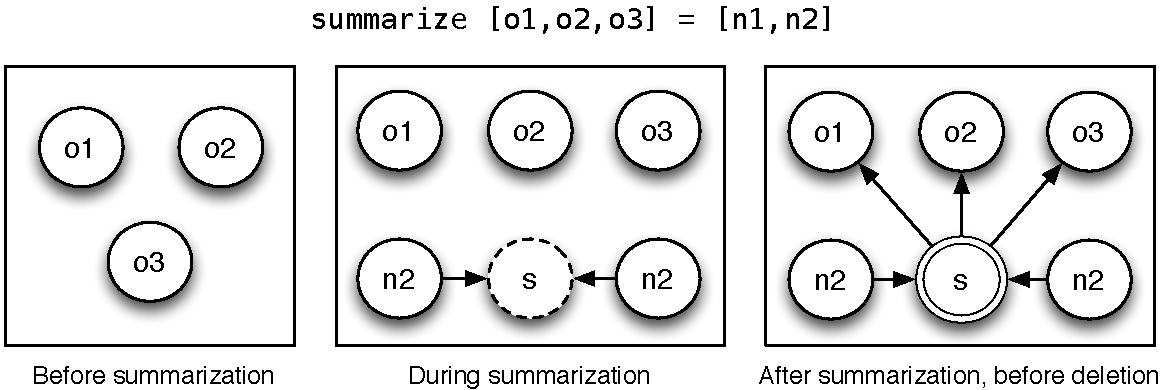
\includegraphics[width=0.8\columnwidth]{Figures/SumDisk}
\end{center}
\caption{Summarization in the backing store. Dotted circle represents effects not yet inserted into the backing store.}
\label{fig:impl_sum_disk}
\end{figure}

To this end, we adopt a novel summarization strategy that builds on the
causality property of the store. Figure~\ref{fig:impl_sum_disk} illustrates the
summarization strategy. Suppose the original set of effects on an object are
$o1$, $o2$ and $o3$. Whe summarized, the new effects yielded are $n1$ and $n2$.
We first instantiate a summarization marker $s$, and similar to transaction
marker, we do not insert it into the store immediately. We insert the new
effects $n1$ and $n2$, with strong consistency, including $s$ as a dependence.
Since $s$ is not yet in the store, the new effects are not made visible to the
clients. Then we insert $s$ with strong consistency, including the original
effects $o1$, $o2$ and $o3$ as dependence. Strongly consistent insertions
ensure that a shim layer node witnessing $s$ on some object must also witness
$n1$ and $n2$ on the same object. A shim layer node which witnesses all the
effects removes the original effects from its cache since they are superseded
by the new effects. Finally, the old effects are deleted from the backing
store. This process ensures that clients either witness the old or the new
effects, but not both; the summarization process appears to be atomic from the
clients perspective.

\section{Evaluation}
\label{q_sec:results}

In this section, we evaluate \quelea programs, report their contract profile
and illustrate the performance benefits of fine-grained consistency
classification on operations and transactions. We also evaluate on the impact
of the summarization. We implemented the following applications, which includes
individual RDTs as well as larger applications composed of several RDTs:

\begin{itemize}

\item \textbf{LWW register}: A last-write-wins register that provides read and
write operations. Each write is associated with a timestamp, which is used to
resolve conflicting concurrent writes -- newer write wins.

\item \textbf{DynamoDB register}: A integer register that allows eventual and
strong puts and gets, conditional puts, increment and decrement operations.

\item \textbf{Bank account}: Our running example, with savings and current
accounts.

\item \textbf{Shopping list}: Collaborative shopping list which allows adding
and deleting items.

\item \textbf{Online store}: Models an online store with shopping cart and
dynamically changing item prices. Checkout process verifies that the customer
only pays the accepted price.

\item \textbf{RUBiS}: An ebay-like auction site~\cite{RUBiS}. The application
allows users to browse items, bid for items on sale, and pay for items from a
wallet modelled after a bank account.

\item \textbf{Microblog}: A twitter-like microblogging site, modelled after
Twissandra~\cite{Twissandra}. The application allows adding a new user, adding
and replying to tweets, following, unfollowing and blocking users, and fetching
a user's timeline, userline, followers and following.
\end{itemize}

\begin{table}[t]
\setlength{\tabcolsep}{4pt}
{\sffamily \small
\begin{center}
\begin{tabular} {|l|r|r|r|r|r|r|r|r|}
\hline
{\bf Benchmark} & {\bf LOC} & {\bf \#T} & {\bf EC} & {\bf CC} & {\bf SC} & {\bf RC} & {\bf MAV} & {\bf RR} \\
\hline
{LWW Reg} & 108 & 1 & 2 & 2 & 2 & 0 & 0 & 0 \\
{DynamoDB} & 126 & 1 & 3 & 1 & 2 & 0 & 0 & 0 \\
{Bank Account} & 155 & 1 & 1 & 1 & 1 & 1 & 0 & 1 \\
{Shopping List} & 140 & 1 & 2 & 1 & 1 & 0 & 0 & 0 \\
{Online store} & 340 & 4 & 9 & 1 & 0 & 2 & 0 & 1 \\
{RUBiS} & 640 & 6 & 14 & 2 & 1 & 4 & 2 & 0 \\
{Microblog} & 659 & 5 & 13 & 6 & 1 & 6 & 3 & 1 \\
\hline
\end{tabular}
\end{center} }
\caption{The distribution of classified contracts. \#T refers to the number of
tables in the application. The columns 4-6 (7-9) represent operations
(transactions) assigned to this consistency (isolation) level.}
\label{tab:ctrts}
\end{table}

The distribution of contracts in these applications is given in
Table~\ref{tab:ctrts}. We see that majority of the operations and transactions
are classified as eventually consistent and RC, respectively. Operation
contracts are used to enforce integrity and visibility constraints on
individual fields in the tables. Transactions are mainly used to consistently
modify and access related fields across tables. In \quelea, the contract
classification process is completely performed at compile time and has no
overheads at runtime. The proof obligations associated with contract
classification is discharged through the Z3 SMT Solver. Across our benchmarks,
classifying a contract took 11.5 milliseconds on average.

For our performance evaluation, we deploy \quelea applications in
\emph{clusters}, where each cluster is composed of 5 fully replicated Cassandra
replicas within the same datacenter. We instantiate one shim layer node for
every Cassandra replica, and place it on the same VM as the Cassandra replica.
Clients are instantiated on the same data center as the store, and run
transactions. We deploy the each node in the cluster on \cf{c3.4xlarge} Amazon
EC2 instances. Our shim layer nodes are multi-threaded, and we allocate 8 CPUs
(out of 16 available) for each shim layer node. The clients also run on
\cf{c2.4xlarge} instances. We call this \cf{1DC} configuration. For our
geo-distributed experiments (\cf{2DC}), we instantiate 2 clusters, each with 5
nodes, and place the clusters on US-east (Virginia) and US-west (Oregon). The
average inter-region latency was 85ms.

\begin{figure*}[t]
  \centering
  \subfigure[Latency]{\label{grf:BA-lat}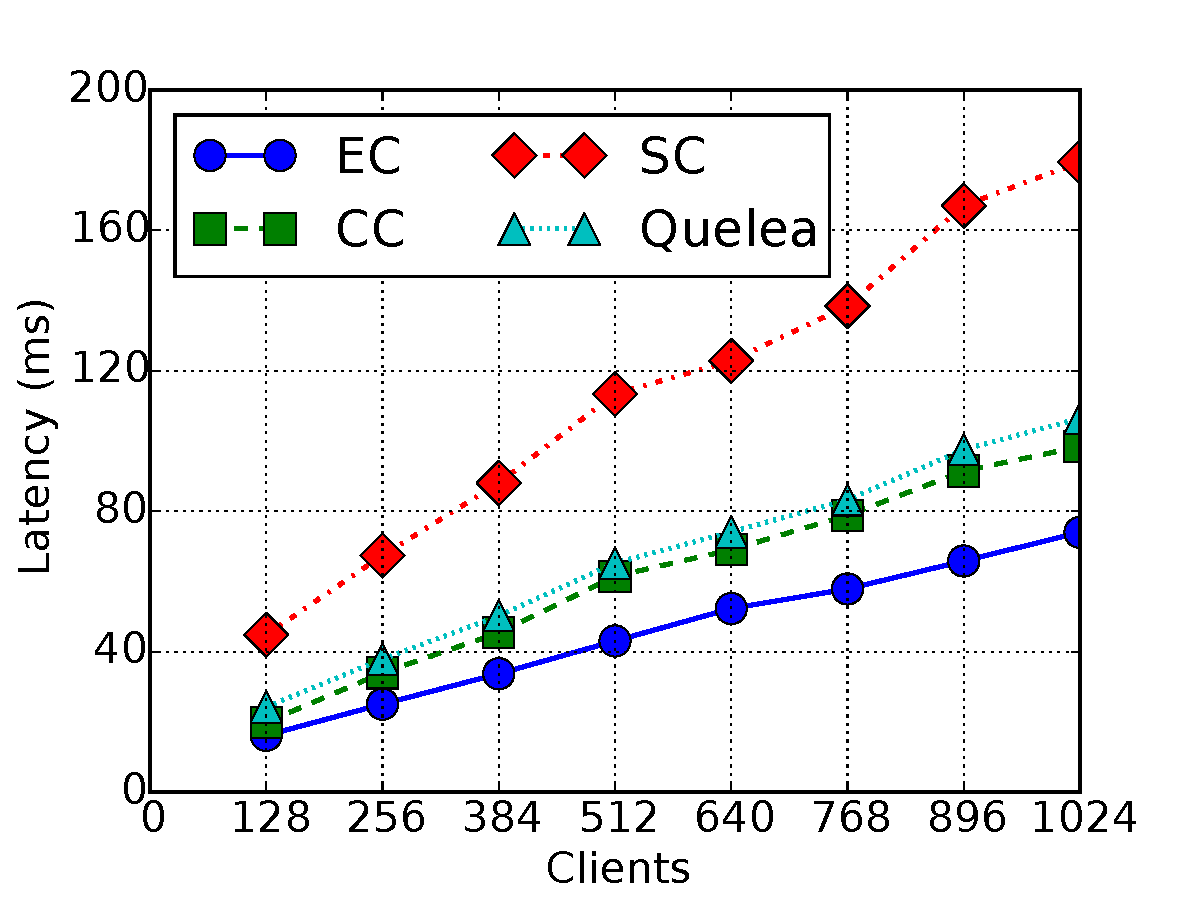
\includegraphics[width=0.45\textwidth]{graphs/BA-lat.pdf}}
  \subfigure[Throughput]{\label{grf:BA-tp}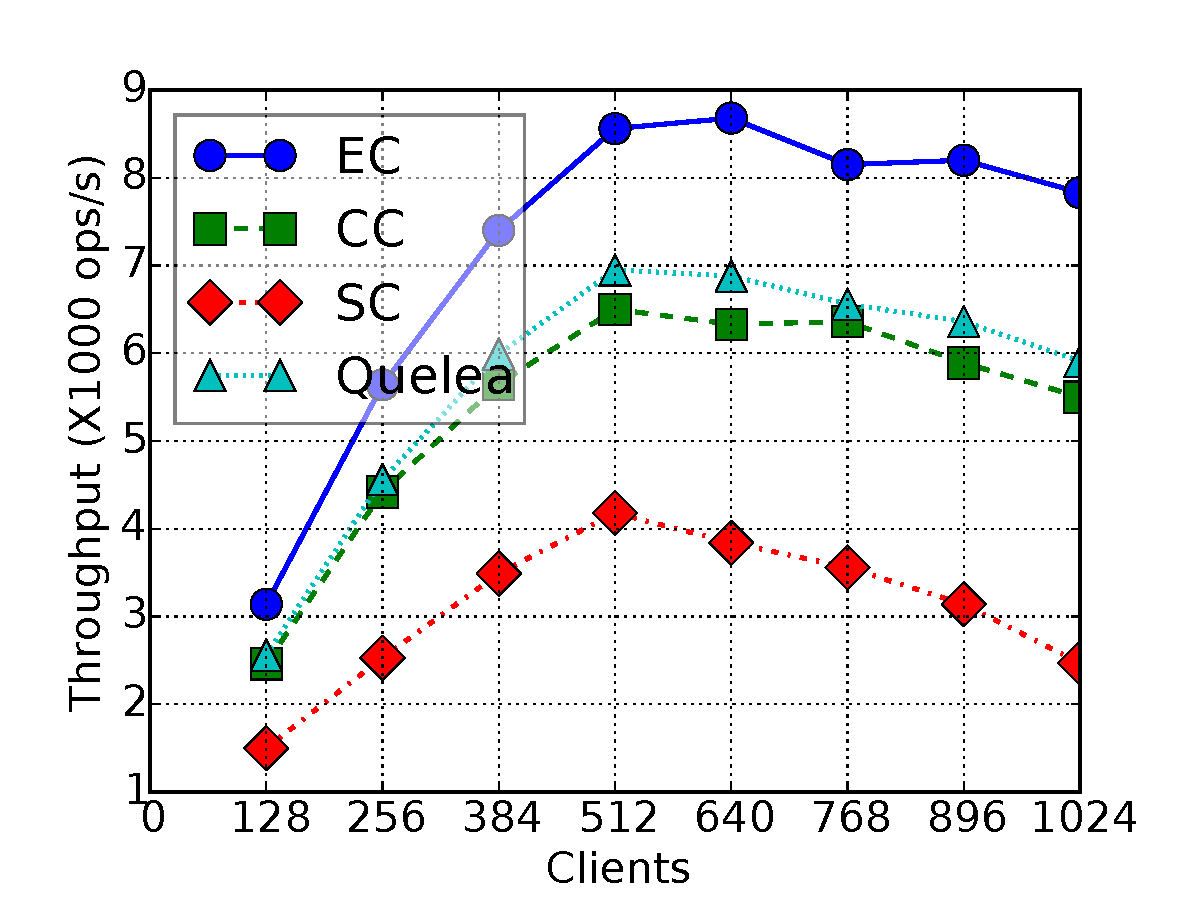
\includegraphics[width=0.45\textwidth]{graphs/BA-tp.pdf}}
  \subfigure[Throughput vs. Latency]{\label{grf:BA-tp-vs-lat}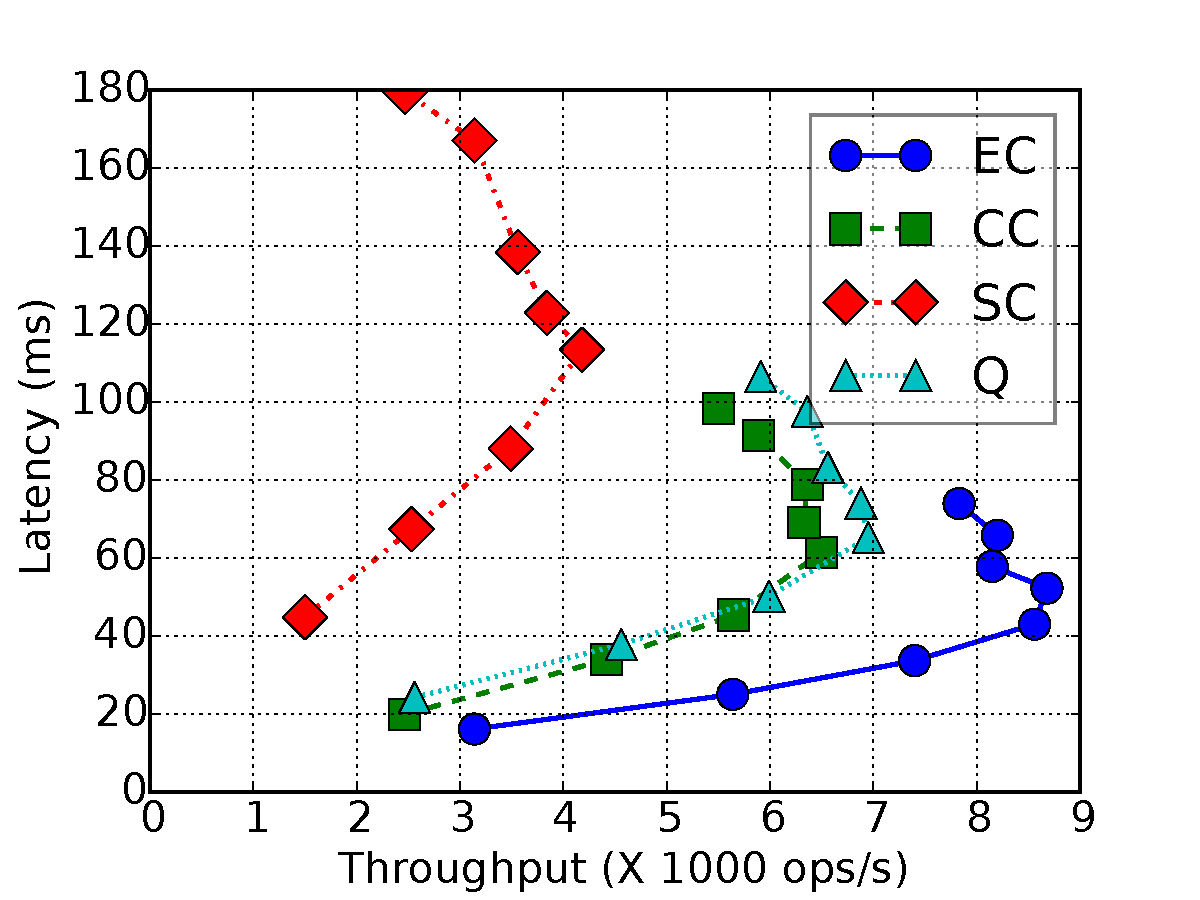
\includegraphics[width=0.45\textwidth]{graphs/BA-tp-vs-lat.pdf}}
	\caption{Bank account performance.}
  \label{grf:BA}
\end{figure*}


Figure~\ref{grf:BA} shows the performance of operations in bank account example
as we increase the number of clients in \cf{1DC} configuration. Our client
workload was generated using YCSB benchmark~\cite{YCSB}. The benchmark
uniformly chose from 100,000 keys, where the operation spread was 25\%
withdraw, 25\% deposit and 50\% getBalance, which corresponds to the default
50:50 read:write mix in YCSB. We increased the number of clients from 128 to
1024, and each experiment ran for 180 seconds.

The lines marked EC and CC correspond to all operations being assigned EC and
CC consistency levels. These levels compromise correctness as withdraw has to
be and SC operation. The line SC corresponds to a configuration where all
operations are strongly consistent; this ensures application correctness.
\quelea corresponds to our implementation, which classifies operations based on
their contracts. Both \quelea and SC ensure correctness. However, with 512
clients, \quelea implementation was within 41\% of latency and 18\% of
throughput of EC, whereas SC operations had 162\% higher latency and 52\% lower
throughput than EC operations. Observe that in the
Figure~\ref{grf:BA-tp-vs-lat} which compares throughput vs. latency, there is a
point in each case after which the latency increases while the throughput
decreases. This indicates a point after which the store becomes saturated with
client requests.

In \cf{2DC} configuration (not-shown), the average latency of SC operations
with 512 clients increased by 9.4$\times$ due to the cost of geo-distributed
coordination, whereas \quelea operations were only 2.2$\times$ slower, mainly
due to the increased cost of \cf{withdraw} operations. Importantly, the latency
of \cf{getBalance} and \cf{deposit} remained almost the same. This illustrates
the benefit of fine-grained contract classification in \quelea.

\begin{figure*}[t]
  \centering
  \subfigure[Latency]{\label{grf:LWW-txn-lat}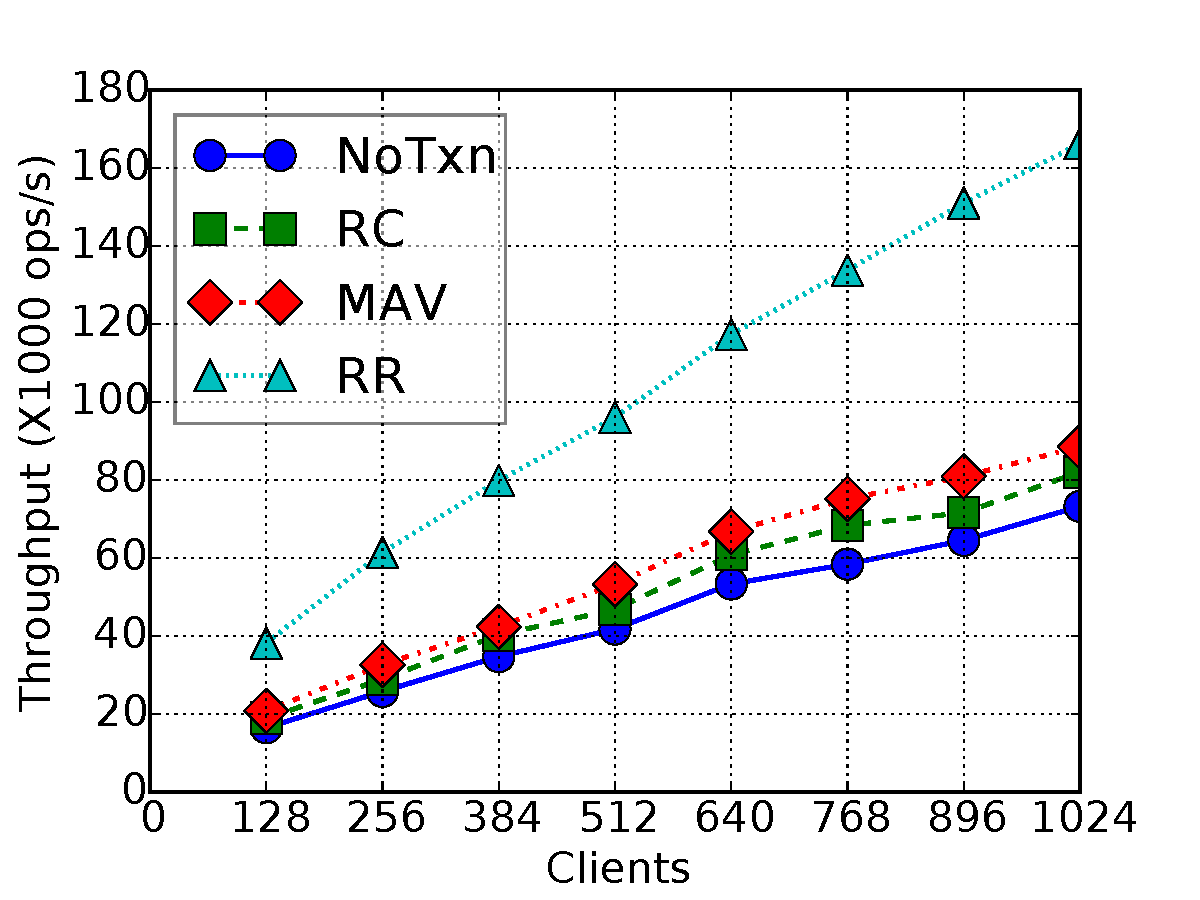
\includegraphics[width=0.45\textwidth]{graphs/LWW-txn-lat.pdf}}
  \subfigure[Throughput]{\label{grf:LWW-txn-tp}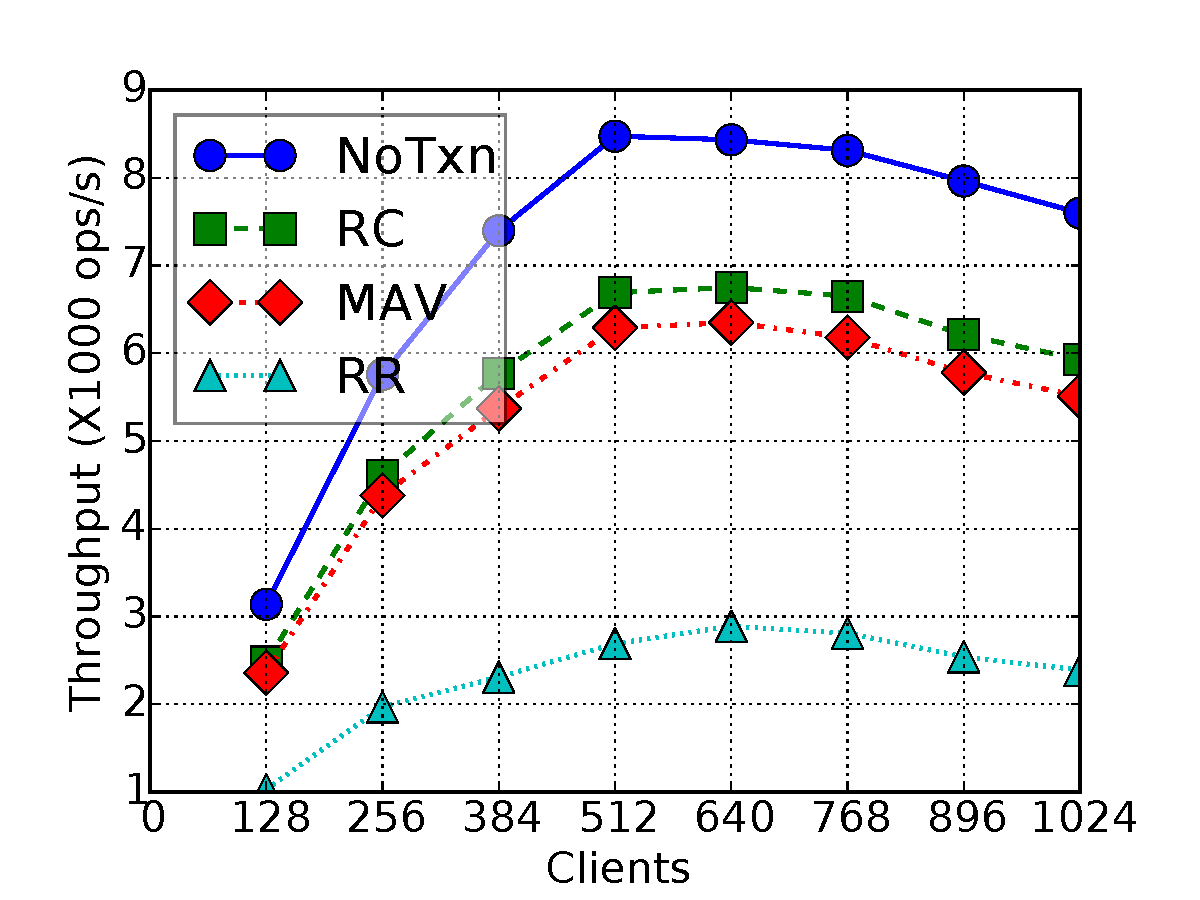
\includegraphics[width=0.45\textwidth]{graphs/LWW-txn-tp.pdf}}
  \subfigure[Throughput vs. Latency]{\label{grf:LWW-txn-tp-vs-lat}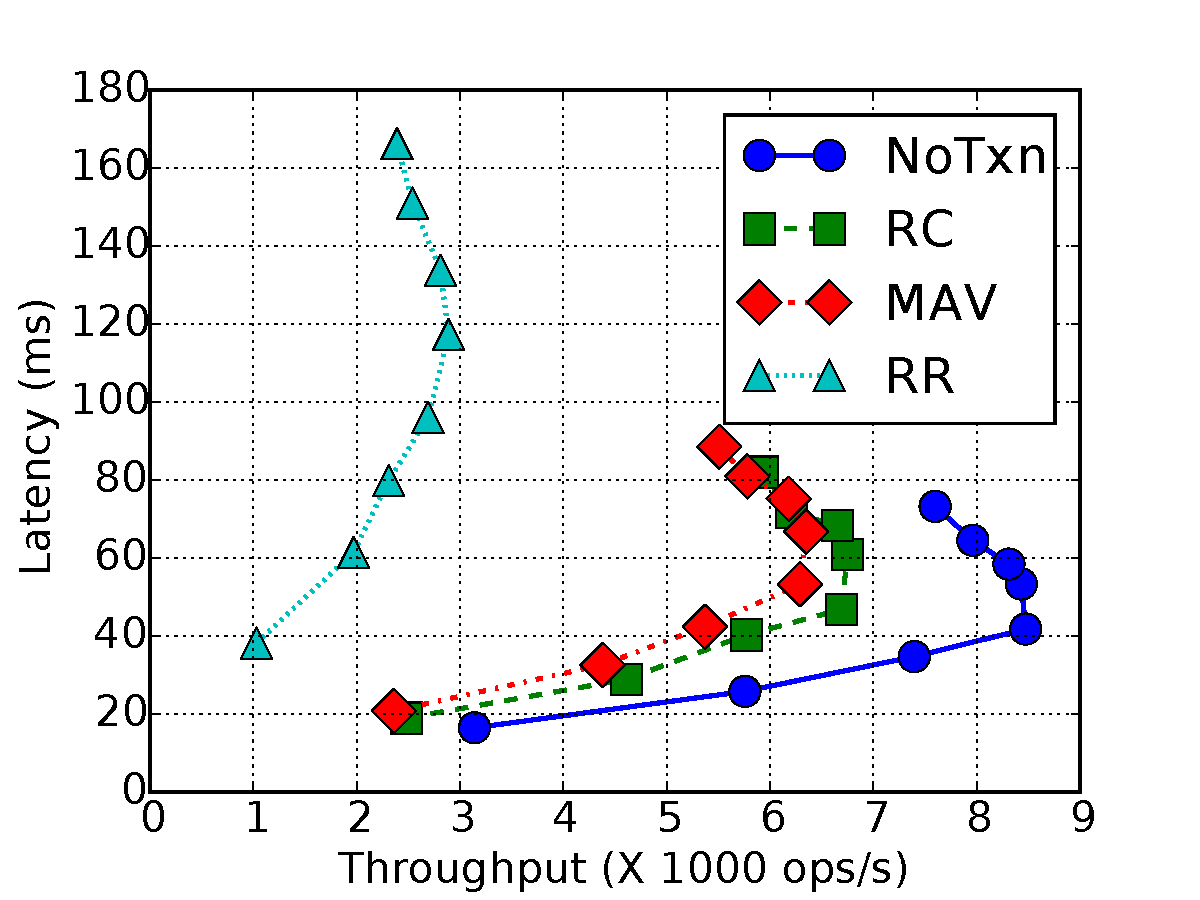
\includegraphics[width=0.45\textwidth]{graphs/LWW-txn-tp-vs-lat.pdf}}
	\caption{LWW register transaction performance.}
  \label{grf:LWW-txn}
\end{figure*}

We compare the performance of different transaction isolation level choices in
Figure~\ref{grf:LWW-txn} using the LWW register. The numbers were obtained
under 1DC configuration. The YCSB workload was modified to issue 10 operations
per transaction, with the default 50:50 read:write mix. Each operation is
assumed to have eventual consistency. \cf{NoTxn} corresponds to a configuration
that does not use transactions. Compared to this RC is only 12\% shower in
terms of latency with 512 clients, where as RR is 2.3X slower. The difference
between RC and \cf{NoTxn} is due to the meta-data overhead of recording
transaction information in the object state. For RR transaction, the cost of
capturing and maintaining the snapshot in an RR transaction is the biggest
source of overhead.

We also compared (not shown) the performance of EC LWW operations directly
against Cassandra (our backing store), which uses last-writer-wins as the only
convergence semantics. While Cassandra provides no stronger-than-eventual
consistency properties, \quelea was within 30\%(20\%) of latency(throughput) of
Cassandra with 512 clients, illustrating that the programmers only have to pay
a minimal overhead for the expressive and stronger \quelea programming model.

\begin{figure}[t]
  \centering
  \subfigure[Latency]{\label{grf:rubis-lat}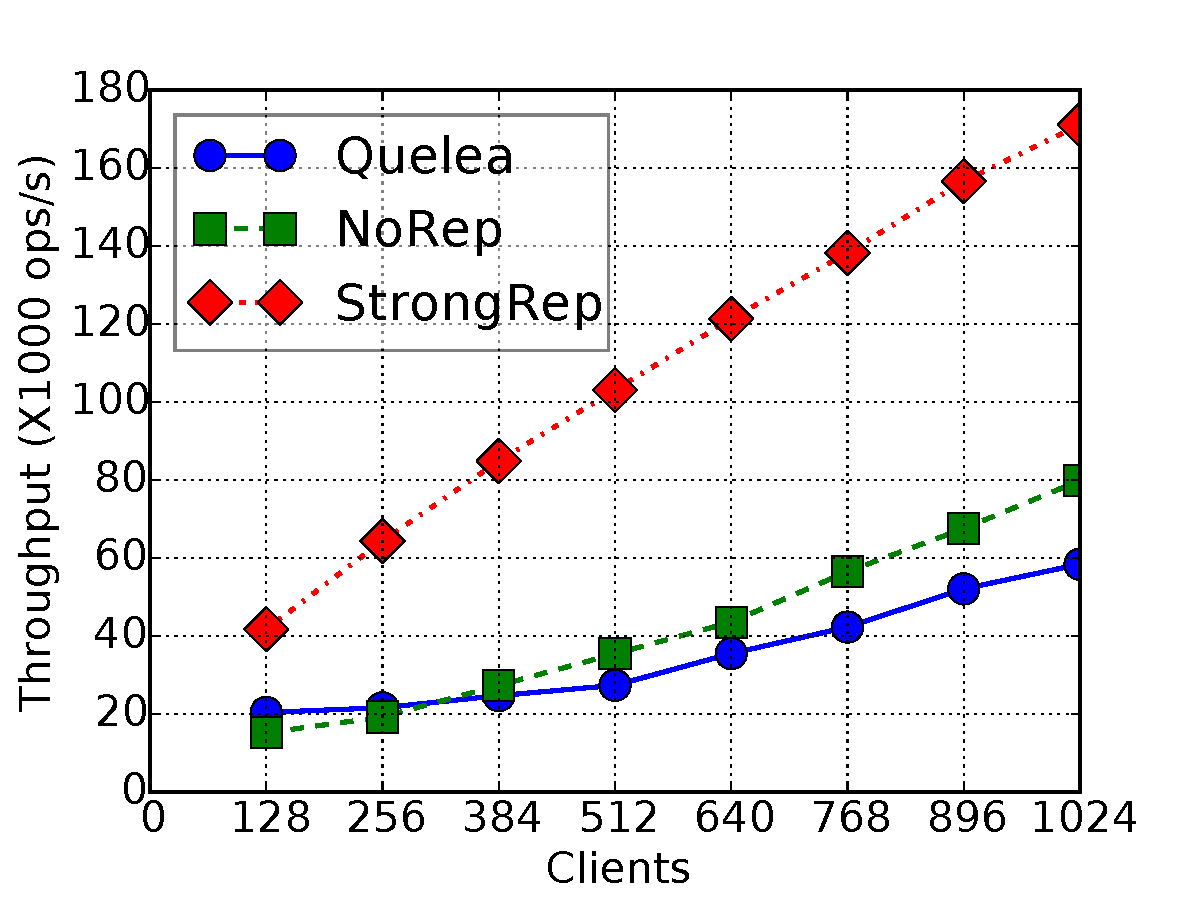
\includegraphics[width=0.45\textwidth]{graphs/Rubis-lat.pdf}}
  \subfigure[Throughput]{\label{grf:rubis-tp}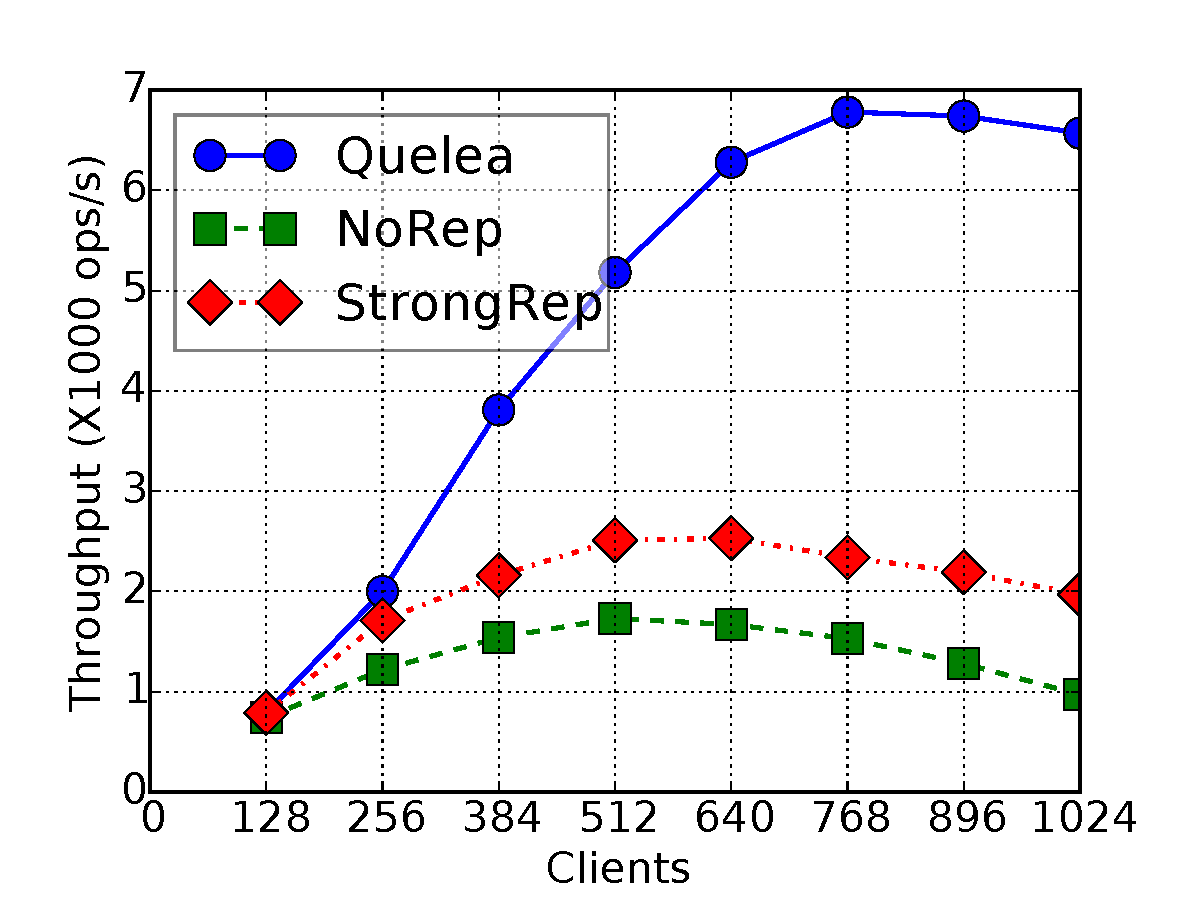
\includegraphics[width=0.45\textwidth]{graphs/Rubis-tp.pdf}}
  \subfigure[Throughput vs. Latency]{\label{grf:Rubis-tp-vs-lat}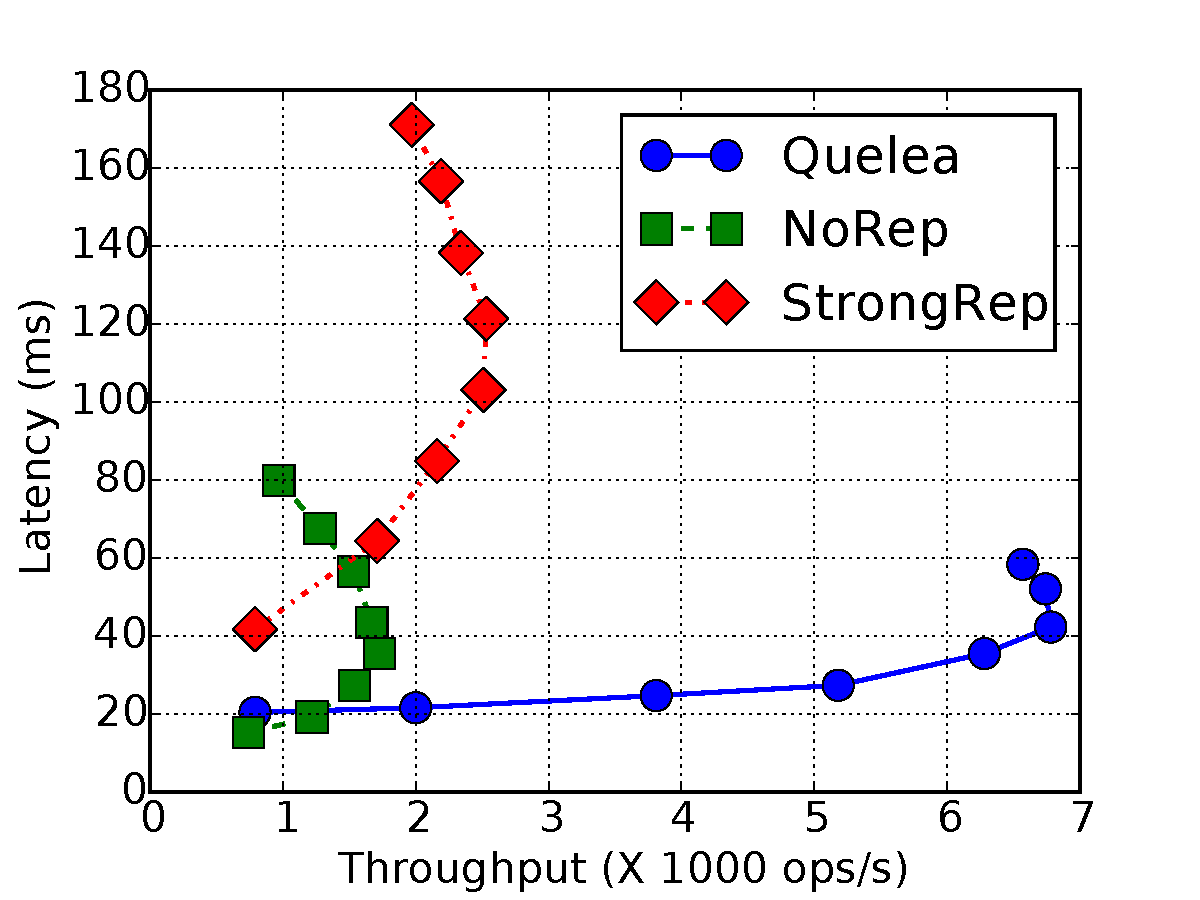
\includegraphics[width=0.45\textwidth]{graphs/Rubis-tp-vs-lat.pdf}}
	\caption{Rubis bidding mix performance.}
  \label{grf:rubis}
\end{figure}


Figure~\ref{grf:rubis} compares the \quelea implementation of RUBiS in \cf{1DC}
configuration against a single replica (NoRep) and strongly replicated
(StrongRep) \cf{1DC} deployment. The benchmark was RUBiS bidding mix, which has
15\% read-write interactions, which is representative of the auction workload.
Without replication, NoRep trivially provides strong consistency. However, this
deployment does not scale beyond 1750 operations per second. Strong replication
offers better throughput at the cost of greater latency due to inter-replica
coordination. \quelea deployment offers the benefit of replication, while only
paying the cost of coordination when necessary.

\begin{figure}[t]
\centering
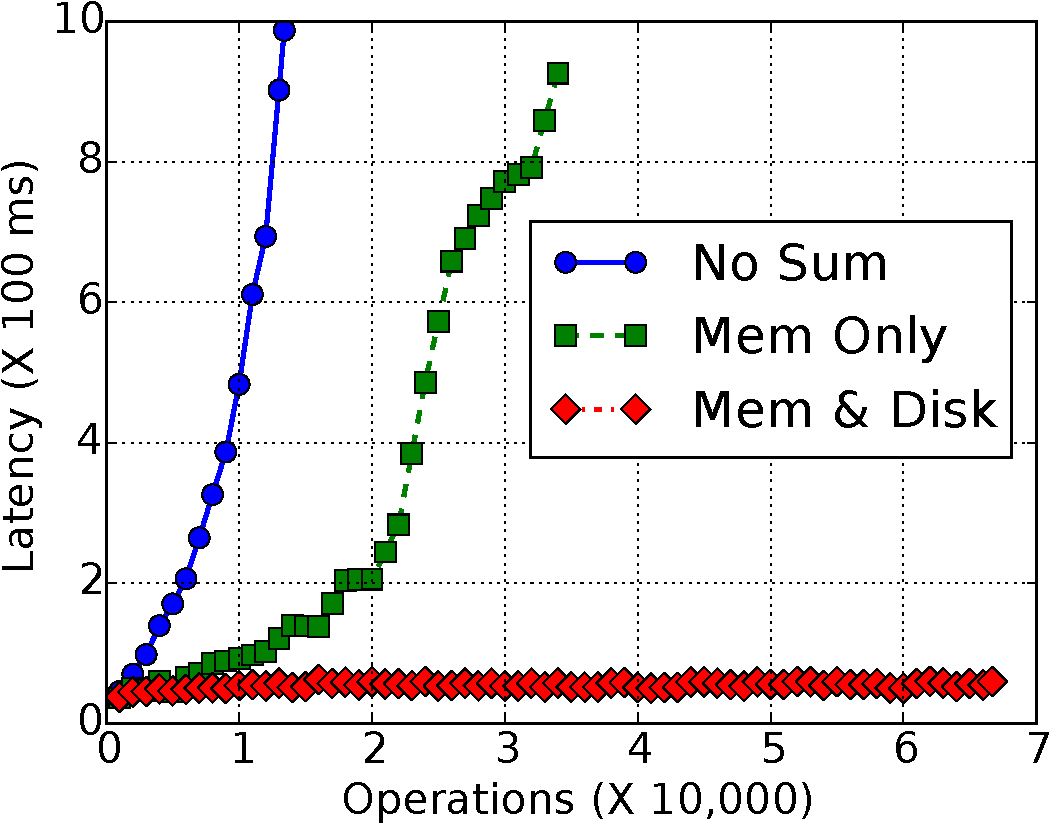
\includegraphics[width=0.45\textwidth]{graphs/summarization.pdf}
\caption{Impact of summarization.}
\label{grf:summarization}
\end{figure}

Finally, we study the impact of summarization in
Figure~\ref{grf:summarization}. We utilize 128 clients and a single \quelea
replica, with all the clients operating on the \emph{same} LWW register to
stress test the summarization mechanism. The shim layer cache (mem) of
operations is summarized every 64 updates, while the updates in the backing
store (disk) are summarized every 4096 updates. Each point in the graph
represents the average latency of the previous 1000 operations. Each experiment
is run for 60s.

The results show that without summarization, the average latency of operations
increase exponentially to almost 1 second, and only 13K operations were
performed in a minute. Since every operation has to reduce over the set of all
previous operations, with a ever growing set, the operations take increasingly
more time to complete. With summarization only in memory, the performance still
degrades due to the cost of fetching all previous updates from the backing
store into the shim layer. Fetching the latest updates is essential for SC
operations. With both summarizations enabled, we see that the latency does not
increase over time, and we were able to perform 67K operations. This graph
illustrates the importance and effectiveness of summarization in \quelea.

\section{Related Work}
\label{q_sec:related}

Operation-based RDTs have been widely studied in terms of their algorithmic
properties~\cite{SSS,Burckhardt2014}, and several systems utilize this model to
construct distributed data structures~\cite{Lakshman2010,Bayou,Tango}. These
systems typically propose to implement the datatypes directly over a cluster of
nodes, and only focus on basic eventual consistency. Hence, these systems
implement custom solutions for durability and fault-tolerance. \quelea realizes
RDTs stronger consistency models on top of off-the-shelf eventually consistent
distributed stores. In this respect, \quelea is similar to~\cite{BoltOn} where
causal consistency is achieved through a shim layer on Cassandra, which
explicitly tracks and enforces dependencies between updates.
However,~\cite{BoltOn} does not support user-defined RDTs, automatic contract
classification and transactions.

Since eventual consistency alone is insufficient to build correct applications,
several systems~\cite{Bayou,Terry2013,RedBlue} propose a lattice of stronger
consistency levels. Similarly, traditional database processing
systems~\cite{Berenson95} and their replicated variants~\cite{BailisHAT}
propose weaker isolation levels for performance. In these systems, the onus is
on the developer to choose the correct consistency(isolation) level for
operations(transactions). \quelea relieves the developer of this burden, and
instead expects contracts expressing declarative visibility requirements.

Our contract language is inspired by the axiomatic description of RDT semantics
proposed by~\cite{Burckhardt2014}. While they use axioms for formal
verification of correctness of an RDT implementation, we utilize them as a
means for the user to express the desired consistency guarantees in the
application. Similar to their work, our contract language does not incorporate
real (i.e., wall-clock) time. Hence, it cannot describe store semantics such as
recency or bounded-staleness guarantees offered by certain
stores~\cite{Terry2013}.

Several conditions have been proposed to judge whether an operation on a
replicated data object needs coordination or not. ~\cite{Calm} defines
\emph{logical monotonicity} as a sufficient condition for coordination freedom,
and proposes a consistency analysis that marks code regions performing
non-monotonic reasoning (eg: aggregations, such as \cf{COUNT}) as potential
coordination points.  ~\cite{IConfluence} and ~\cite{Sieve} define
\emph{invariant confluence} and \emph{invariant safety}, respectively, as
conditions for safely executing an operation without coordination. ~\cite{Sieve}
also proposes a program analysis that conservatively marks operations as
\emph{blue} (coordination not required), while marking the remaining as
\emph{red} (coordination required). Unlike \quelea, these works focus on a
coarse-grained classification of consistency as eventual or strong, and do not
focus on transaction isolation levels. However, program analyses they propose
relieve programmers of the burden to tag operations with consistency levels.
Indeed, we do consider automatic inference of consistency contracts from
application-specific integrity constraints as the next step for \quelea.

\section{Conclusions}
\label{q_sec:concl}

In this chapter, we have presented \quelea a shallow Haskell extension for
declarative programming over eventually consistent data stores. The key idea of
\quelea is the automatic classification of fine-grained consistency contracts on
operations and distributed transactions with respect to the consistency and
isolation levels offered by the store. Our contract language is carefully
crafted from a decidable subset of first-order logic, enabling the use of
automatic theorem prover to discharge the proof obligations associated with
contract classification. We realize an instantiation of \quelea on top of
off-the-shelf distributed store, Cassandra, and illustrate the benefit of
fine-grained contract classification by implementing and evaluating several
scalable applications.
